\documentclass[a4paper, 10pt ]{article}     

% The following packages can be found on http:\\www.ctan.org
\usepackage{graphics} % for pdf, bitmapped graphics files
\usepackage{epsfig} % for postscript graphics files
\usepackage{mathptmx} % assumes new font selection scheme installed
\usepackage{times} % assumes new font selection scheme installed
\usepackage{amsmath} % assumes amsmath package installed
\usepackage{amssymb}  % assumes amsmath package installed
\usepackage[usenames]{color}
\usepackage[utf8]{inputenc} 
\usepackage{algorithm}
\usepackage{algorithmic}

\begin{document}

\begin{center}
\vspace{0.2cm}
\Large \bf{Etude de la marche avec un appui mobile contrôlé}\\
\textit{\bf{Modélisation de la marche d'une personne avec un déambulateur}}\\
\end{center}

\section{Introduction}

Ces travaux poursuivent deux objectifs : 
\begin{itemize} 
\item concevoir un système d'assistance à la locomotion qui permette un suivi quotidien de paramètres pour l'évaluation de la fragilité et le suivi de certaines pathologies ; 
\item concevoir un système d'assistance à la locomotion qui permette de rétablir l'équilibre d'une personne en cours de marche. 
\end{itemize} 

Dans un premier temps, nous nous focaliserons sur l'études des paramètres qui décrivent l'équilibre pour aller vers ces deux objectifs : quantifier la fragilité et améliorer l'équilibre. \\

Le système envisagé se base sur l'instrumentation d'un déambulateur médical à roue de type "rollator", dans la lignée des déambulateurs ANG développés à l'INRIA de Sophia. \\

Nous limiterons l'équipement au système en évitant au maximum d'équiper la personne afin que l'utilisation du déambulateur soit la plus simple possible. Le seul contact entre la personne et l'assistance est un contact entre les mains et deux poignées. \\%//Equipé de capteurs, ce système peut également permettre un suivi au quotidien des utilisateurs et de l'évolution de certaines pathologies.  \\

Les publics visés sont des personnes nécessitant une assistance permanente (personnes agées ou handicapées) ou une assistance temporaire (personnes en cours de rééducation du membre inférieur). \\

Le développement de cette assistance à la locomotion soulève un certain nombre de questions :  
%Pour parvenir à cet objectif, je propose dans un premier temps d'étudier la marche d'une personne avec un appui mobile dont le mouvement est contrôlé. 
\begin{itemize}

%\item Le déambulateur est contrôlé de sorte à réguler une tâche. Quelle tâche que doit on réguler pour maintenir l'équilibre ? Pour répondre à ces questions, on doit d'abord établir quel critère garantit la stabilité du système ? Quelles sont les mesures nécessaire à l'estimation en ligne de de critère ? Quelles mesures sont accessibles sans équiper la personne ni l'environnement ? Positions des pieds ? Force sur les poignées ? Forces de contact ? Posture ?  Peut on se contenter de capteurs embarqués sur le déambulateur ou faut il forcément embarquer les capteurs sur la personne ?

\item Comment modéliser l'équilibre entre une personne et un déambulateur ? % Comment modéliser l'équilibre dynamique de la marche avec un appui mobile dont le déplacement est contrôlé ? 
 %Le système comporte deux sous systèmes (homme et déambulateur) et une liaison à modéliser. Du point de vu logiciel, nous pouvons nous appuyer sur les développements récents de moteurs dynamiques open source (xde du CEA, bibliotheque python arboris de l'ISIR, bibliotheque scilab HUMANS de l'INRIA, openHRP de l'AIST,  bibliothèque du LAAS, bibliothéque de génération de mouvement multicontact du LIRMM ).
 
 \item Est ce que l'utilisation d'un déambulateur perturbe la posture et la marche de la personne ? Peut on encore quantifier des indices de fragilité pertinent en utilisant le déambulateur ou son usage rend l'analyse impossible ?

 
 \item Quel est le jeu de paramètres minimal à observer pour estimer l'état d'équilibre de la personne ? Avec quels capteurs ?

\item Quel est le paramètre à réguler dans la loi de commande du déambulateur pour maintenir la stabilité du système homme-déambulateur ?

\item Quelles sont les expériences à mettre en place pour établir ce critère d'équilibre empiriquement ou le valider expérimentalement ? Nous avons à notre disposition le matériel de l'équipe Handibio et le matériel des équipes Coprin et Arobas, c'est à dire des déambulateurs, des systèmes d'analyse du mouvement (motion capture, plateformes de force, systèmes à câbles), des tapis de marche, une plateforme de stewart

\item Pourra t'on trouver une méthode suffisamment générique pour qu'elle s'adapte à tous les utilisateurs ? Ou bien, faudra-t-il adapter le modèle au type de handicap ou encore à chaque personne ?  Quels sont les paramètres à régler ? Comment les adapter ?

%\item Quels sont les forces à appliquer pour rétablir l'équilibre ?  Comment doit on actionner le déambulateur ? Faut il modifier le déambuleur pour parvenir à stabiliser l'équilibre, par exemple en ajoutant des degrès de liberté dans les poignées ? 

\end{itemize}


Dans ce mémo, nous allons nous intéresser à une première modélisation dans le plan sagital du système homme déambulateur. 

\begin{figure}[h]
\centering
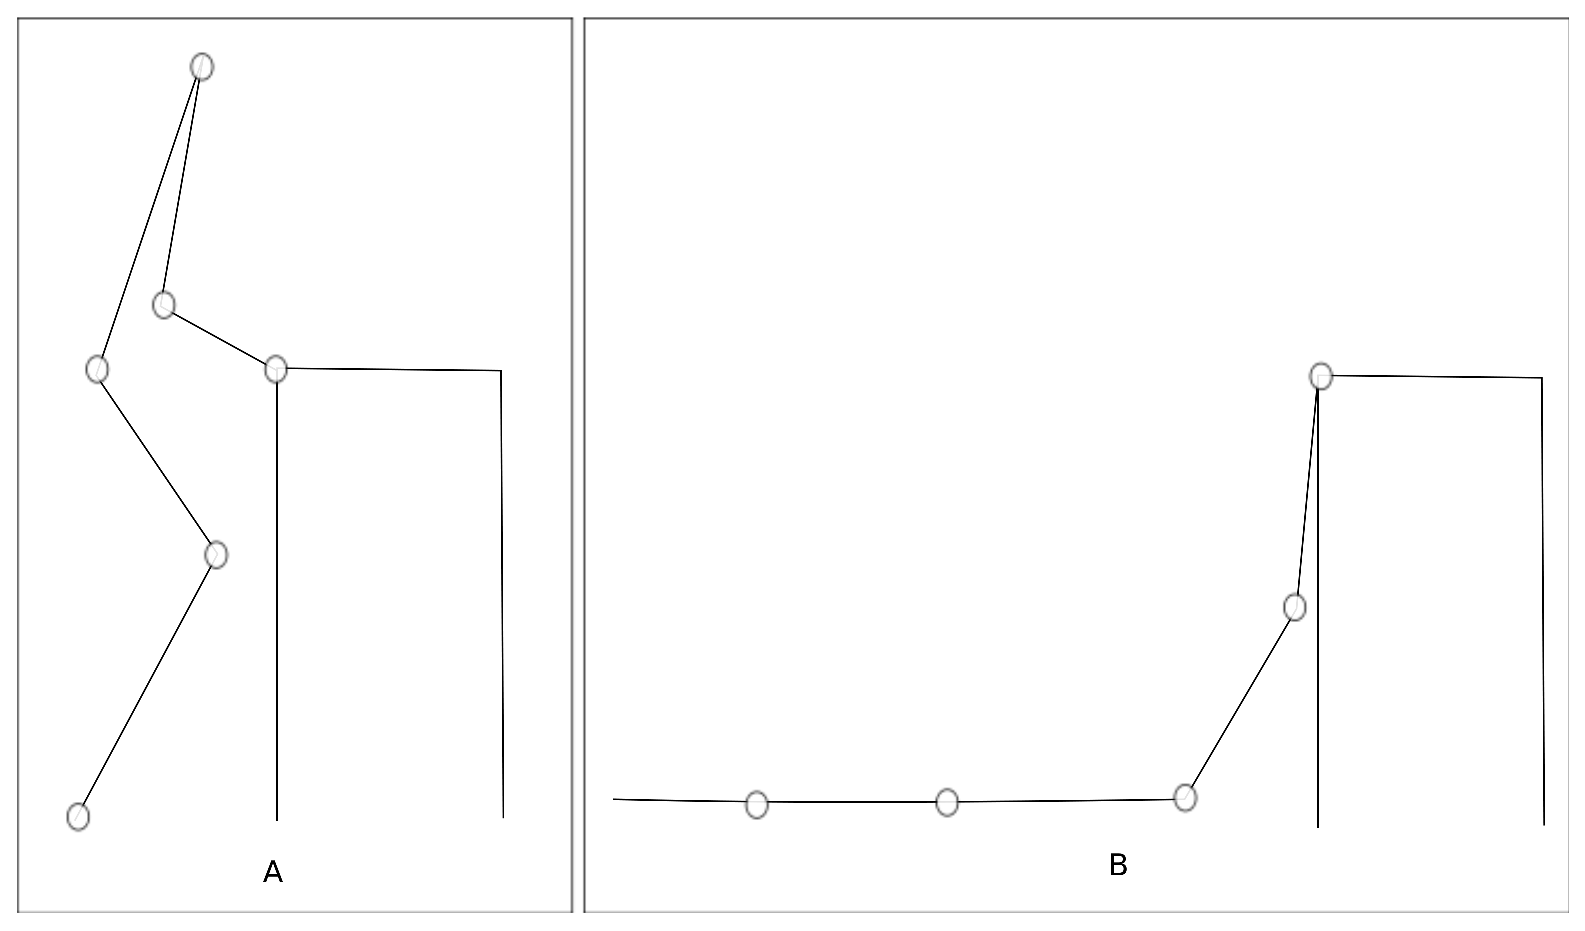
\includegraphics[width=0.6\columnwidth]{images/model/positionStable.eps}
\caption{2 configurations stables du système complet homme-déambulateur}
\label{fig:positionEquilibre}
\end{figure}


Nous expliciterons ensuite ce qu'est l'état d'équilibre du système homme-deambulateur. La figure \ref{fig:positionEquilibre} montre deux états d'équilibre, au sens de la mécanique, du système complet homme-déambulateur. Dans la première configuration, la personne est debout, dans la seconde, elle est couchée au sol suite à une chute. On voit bien que ce qu'on cherche à obtenir n'est pas un état stable du système total mais un état stable pour chacun des sous-systèmes homme et  déambulateur tout en tenant compte de leurs interactions.


Puis, nous proposerons une premiere loi de commande pour maintenir l'équilibre du système.

A chaque étape, et pour chaque modèle, nous mentionnerons les paramètres qui doivent être connus a priori et ceux qui doivent être observés pour pouvoir estimer l'état du système.

\section{Modélisations géométriques et cinématiques}

\subsection{Modèle de l'environnement}

Dans un premier temps, on va supposé que le système évolue sur un sol plan parfaitement horizontal. Cette hypothèse permet de supposer que les appuis des pieds et du déambulateur sont coplanaires et que les forces induites par le poids ont uniquement une composante vertical. 

Il est possible de lever cette hypothèse. Nous y veillerons dans un second temps, en particulier pour pouvoir assister la personne dans des pentes.

\subsection{Modèle du déambulateur}

%\subsection{Critère d'un bon déambulateur (pour info)}
%\noindent (\textit{ source : www.tousergo.com}).
%\begin{itemize}
%\item La largeur et l’aspect pratique. Le déambulateur ne doit pas être trop large pour pouvoir franchir les portes et les couloirs étroits.
%\item Les poignées doivent se trouver à la hauteur des hanches, ou plus exactement à hauteur du pli du poignet lorsque les bras sont relachés le long du corps.
%\item Le poids. Le déambulateur doit être assez léger et facile à manipuler.
%\item  La possibilité d’ajouter des accessoires (un plateau, un panier, un siège...)
%\item Des freins maniables et des roues facilement dirigeables.
%\end{itemize}
%\subsection{Maintenir un faible coût (pour info)}
%
%Pour que le système développé puisse toucher un public large, il faut minimiser son coût. Pour information, les Déambulateurs sont remboursés par la Sécurité Sociale à hauteur de 53,81 euros (Code LPPR 1285619).
%\subsection{Modèle du déambulateur}

Le déambulateur est modélisé comme un ensemble rigide. Seule la hauteur et l'orientation des poignées peut changer pour s'adapter à la taille de la personne en début d'expérience. Dans les faits, lorsqu'une personne s'appuie sur le déambulateur, on constate une légère déformation de la structure que l'on néglige ici. 

On suppose que les roues du déambulateur touchent le sol et que les poignées sont parallèles au plan du sol. On suppose donc que le déambulateur est en appui plan sur le sol et ne peut se déplacer qu'en translation sans se renverser (voir le modèle sur la figure \ref{fig:modelWalker} )

\begin{figure}[h]
\centering
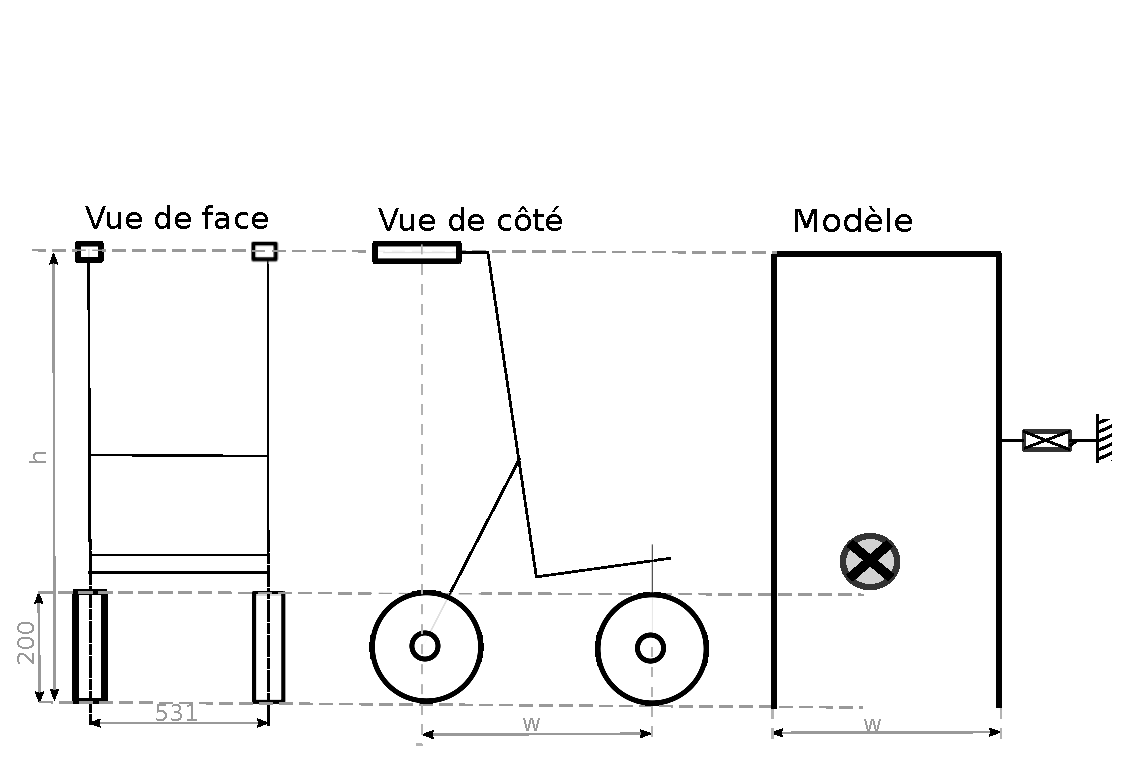
\includegraphics[width=0.6\columnwidth]{images/model/modeleDeambulateur.eps}
\caption{Modélisation du déambulateur à 4 roues}
\label{fig:modelWalker}
\end{figure}

\subsection{Modèle du corps humain}

Le corps humain est modélisé comme un système polyarticulé de corps rigides. Les articulations sont supposées idéales.

Les masses d'inertie et les longueurs des segments sont tirées de tables classiques pour un homme jeune ($<60ans$). Ces données sont erronées pour des personnes âgées mais serviront en première approximation pour établir les premiers critères de stabilité. Ces mêmes données ne sont pas disponible pour des personnes de plus de 60 ans. Il faudra donc adapter ces données aux personnes ou simplifier le modèle pour ne pas en avoir besoin. On peut noter que des travaux récents \cite{Venture12} permettent d'évaluer en ligne les matrices d'inertie et les centre d'inertie d'un sujet en suivant ses mouvements avec un système de motion capture et en mesurant les forces de contact au sol.

\subsubsection{Trois modélisations}

Les figures \ref{fig:ModelHuman38}, \ref{fig:ModelHuman7} et  \ref{fig:ModelHuman4} présentent 3 modèles du corps humain, Human38, Human7 et Human4, de plus en plus simplifié. Dans un premier temps, nous utiliserons le modèle sagital à 7 articulations, Human7, et nous comparerons les résultats obtenus avec un modèle sagital à 4 articulation,Human4, proposé par Ludovic Saint-Bauzel~\cite{Saint-Bauzel2009} dans son manuscrit de thèse.


\begin{figure}[h]
\centering
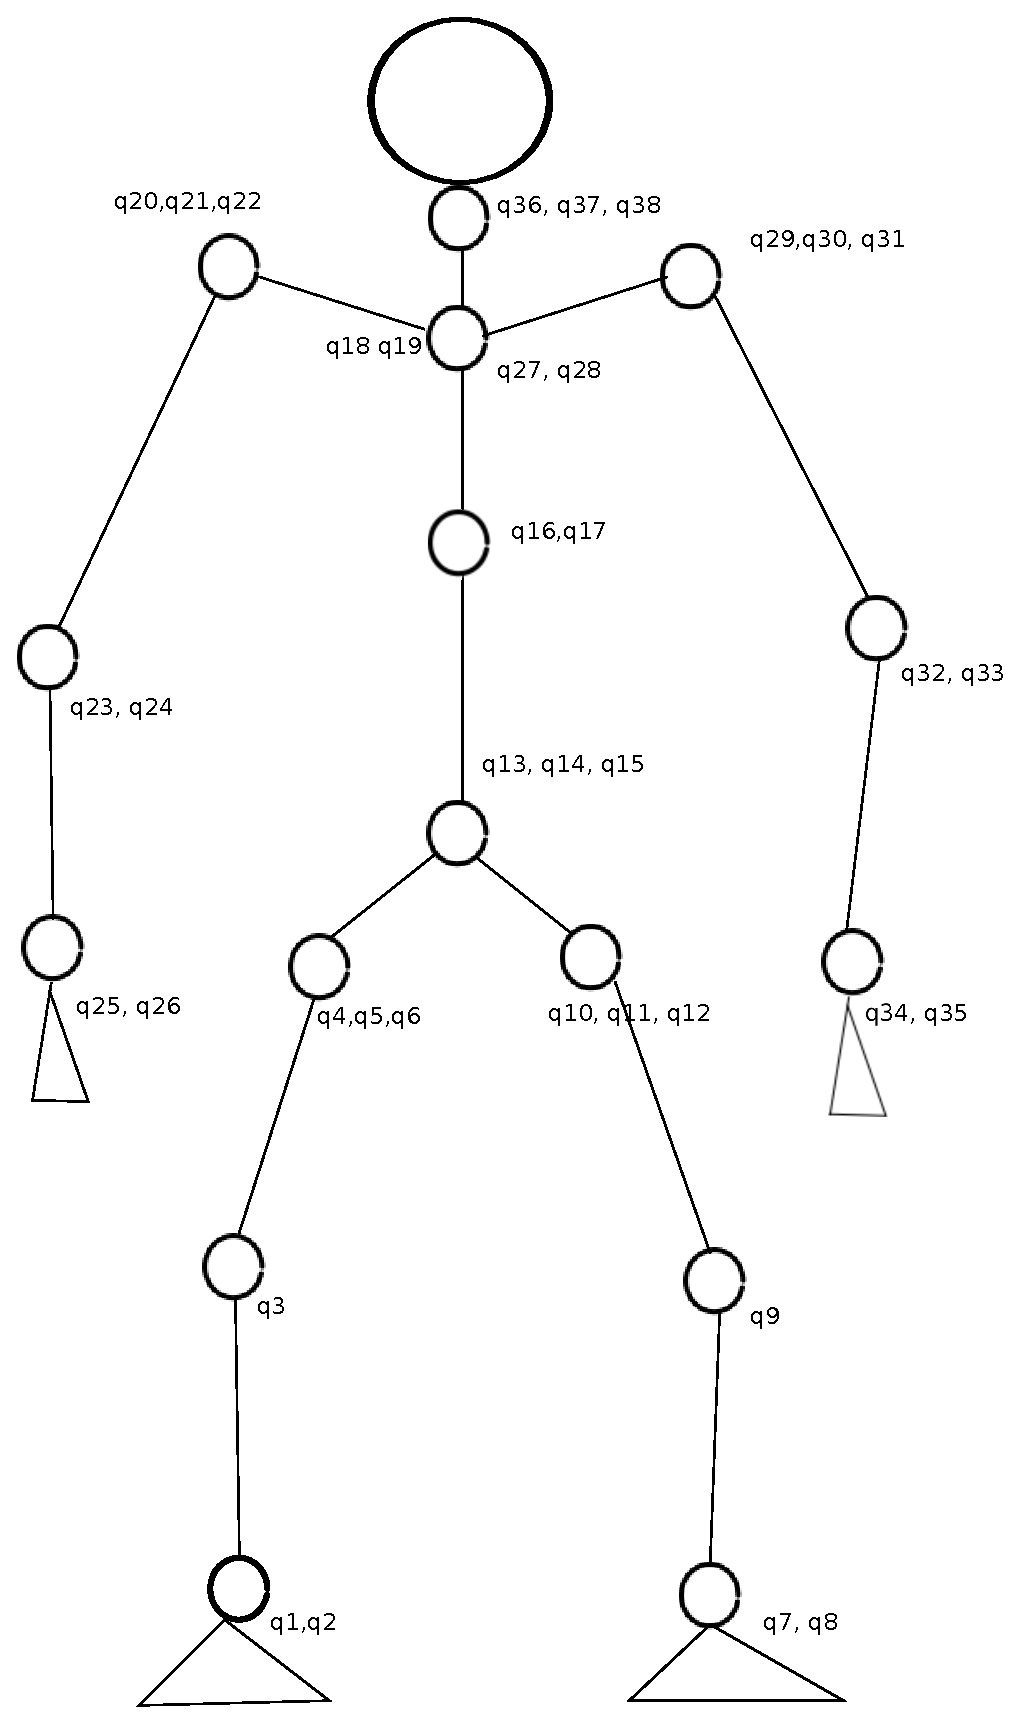
\includegraphics[width=0.6\columnwidth]{images/model/modeleHommeQ.eps}
\caption{Modélisation du corps humain à 19 segments et 38 degrès de liberté. }
\label{fig:ModelHuman38}
\end{figure}

\begin{figure}[h]
\centering
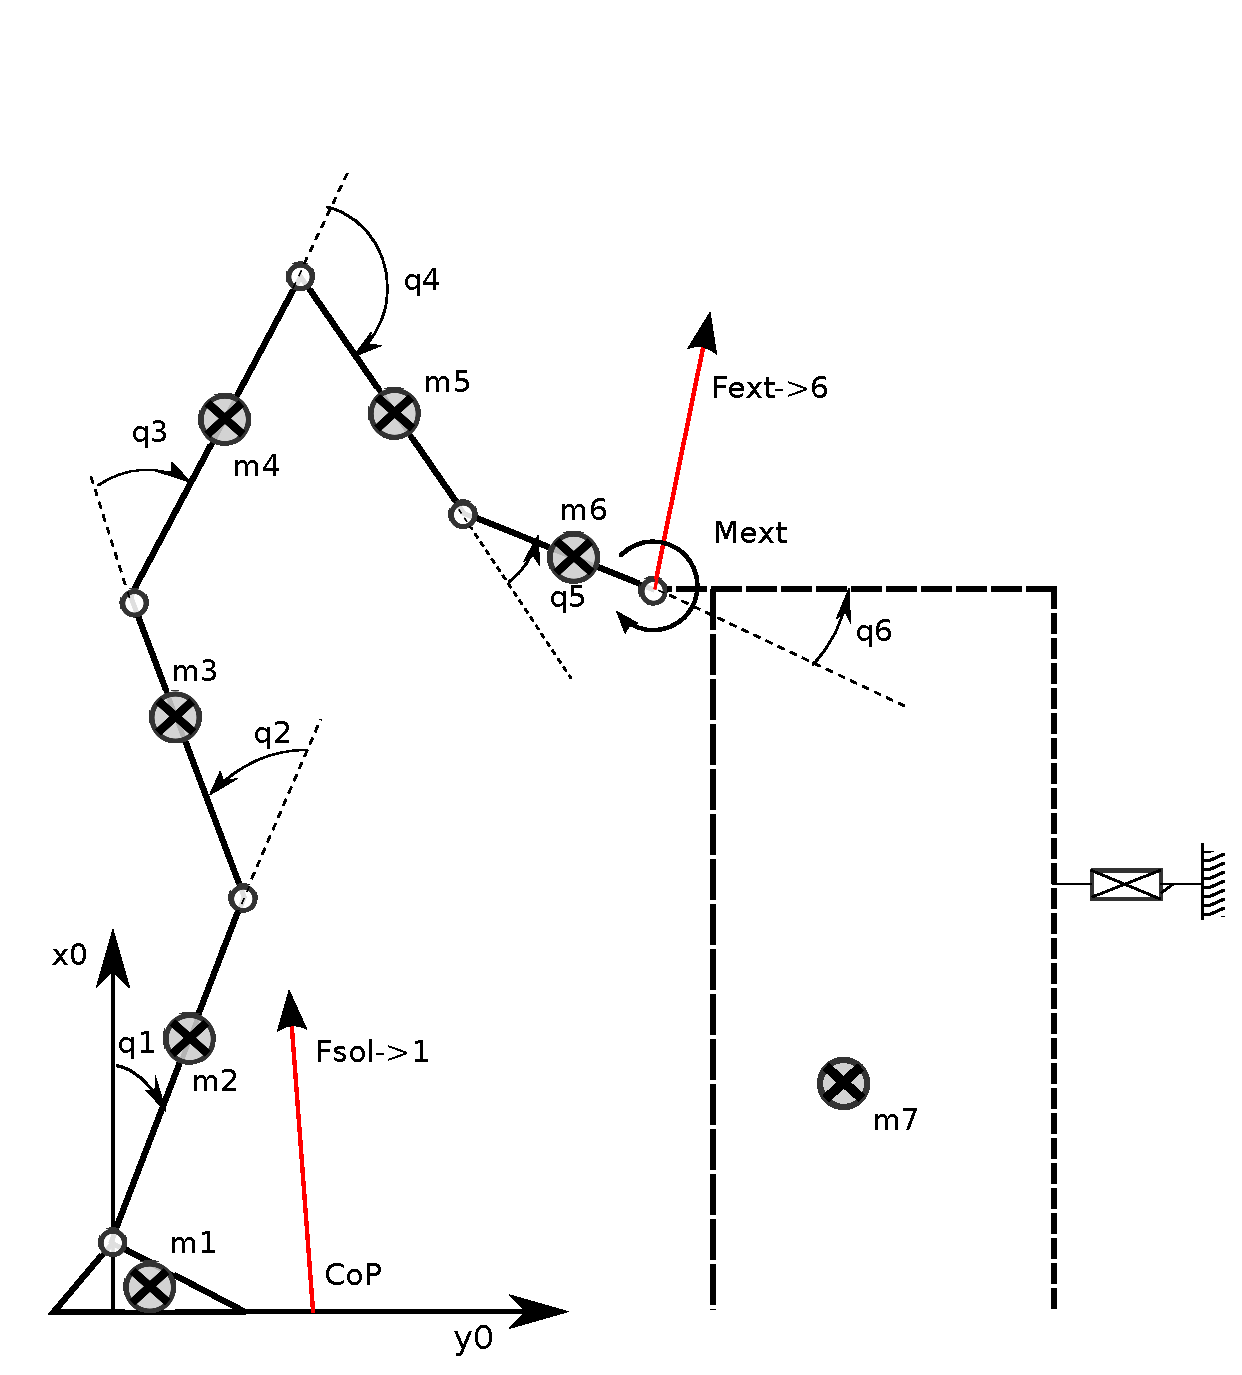
\includegraphics[width=0.6\columnwidth]{images/model/modeleHommeQ7.eps}
\caption{Modélisation du corps humain à 5 segments et 6 degrès de liberté. }
\label{fig:ModelHuman7}
\end{figure}

\begin{figure}[h]
\centering
\includegraphics[width=0.6\columnwidth]{images/model/modeleHommeQ7simple.eps}
\caption{Modélisation du corps humain à 3 segments et 4 degrès de liberté. Modele extrait de la thèse de Ludovic Saint Bauzel ~\cite{Saint-Bauzel2009} sur le levé de personne.}
\label{fig:ModelHuman4}
\end{figure}



Dans la suite de ce document, nous allons utiliser le modèle à 7 degrés de liberté décrit par la figure \ref{fig:ModelHuman7}.
Les modèlisations géométriques et cinématique sont détaillées en annexes \ref{Annexe1} et \ref{Annexe2}. La figure \ref{fig:ModelHuman7GM} décrit la position des repères.

\begin{figure}[h]
\centering
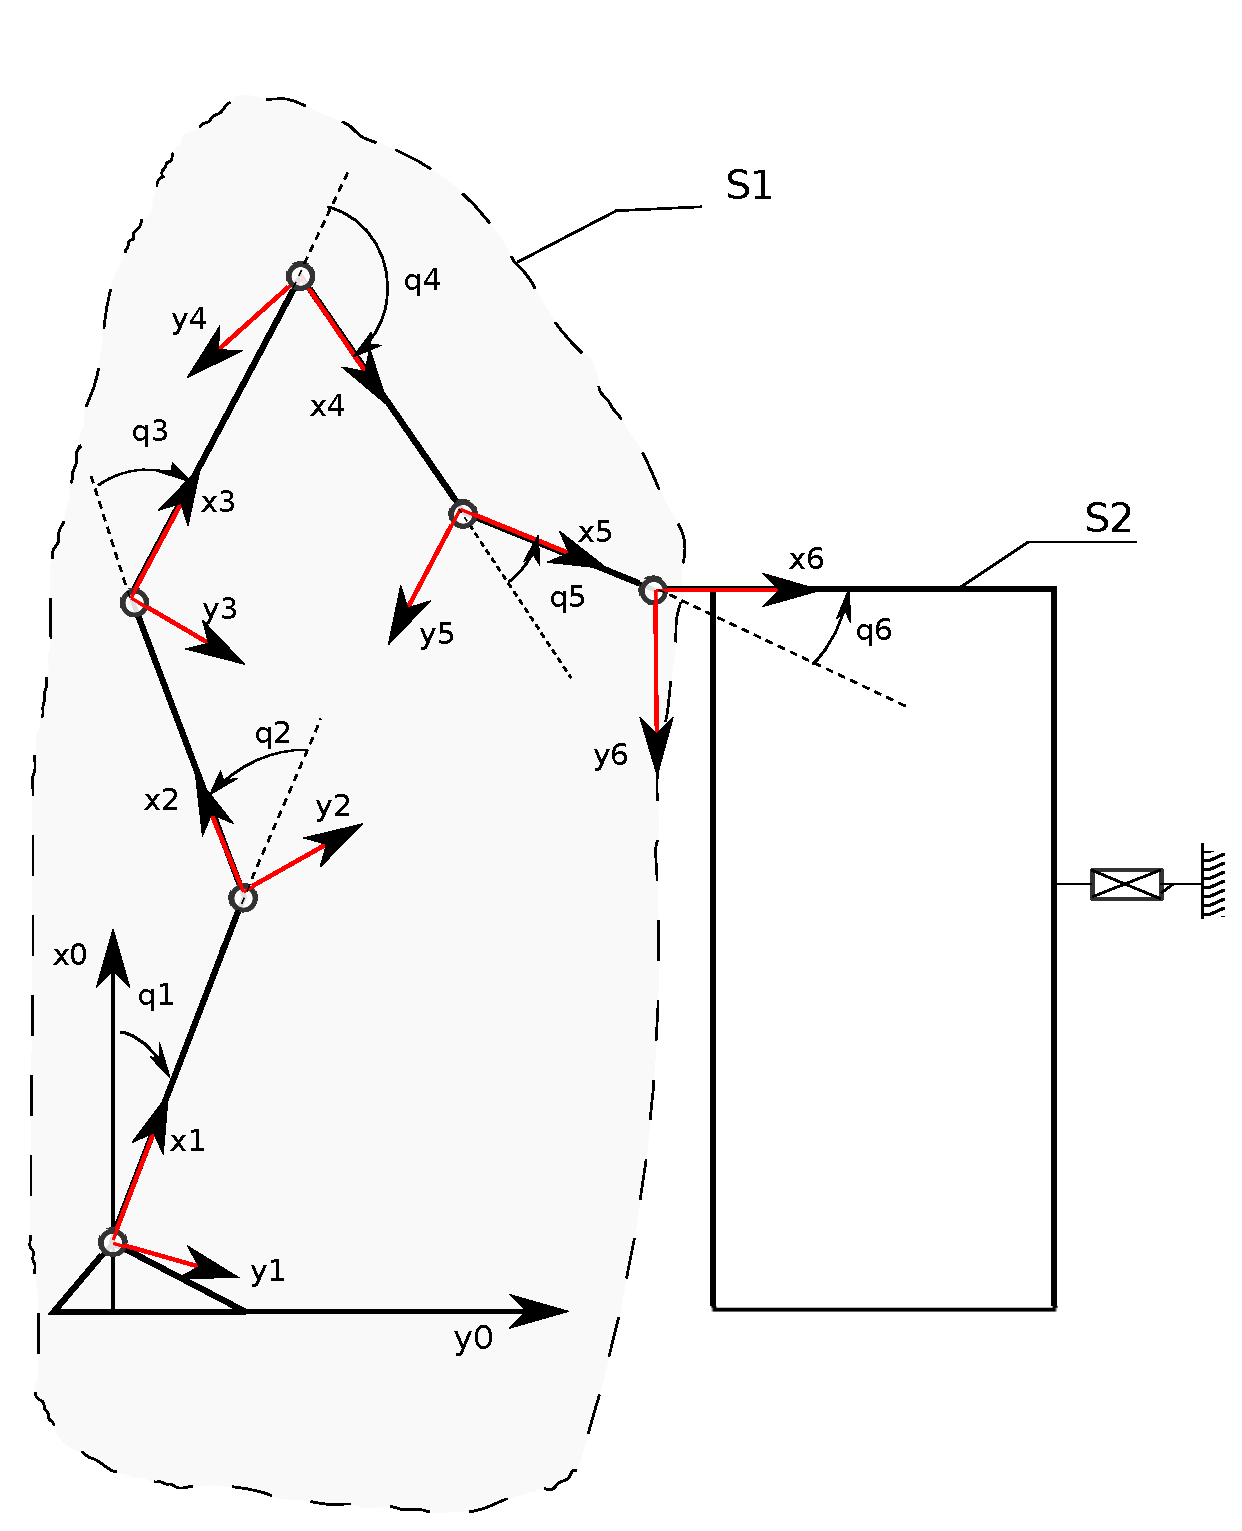
\includegraphics[width=0.5\columnwidth]{images/model/modeleHommeQ7MG.eps}
\caption{Modélisation géométrique du corps humain à 5 segments et 6 degrès de liberté.}
\label{fig:ModelHuman7GM}
\end{figure}

\subsubsection{Longueur des segments}
Les données sont extraites de Dumas et al. \cite{Dumas07} pour un homme en bonne santé de moins de $60$ ans.

\begin{center}
\small{
\begin{tabular}{l |c |c| c| c| c| c|c}
membre & $d_i$ & dimension (m)\\
\hline
pied 	(sol-maleole)		& $d_1$&0.1\\
jambe 			& $d_2$&0.433\\
cuisse 			& $d_3$&0.432\\
tronc			& $d_4$&0.477\\
bras				& $d_5$&0.271\\
avant-bras	&$ d_6$ &0.283\\
\end{tabular}}
\end{center}





\subsubsection{Limites articulaires}

Les amplitudes articulaires sont extraites de l'American Academy of Orthopaedic Surgeons (voir le livre de Allard et al\cite{Allard11}, p34). Ces mesures sont à adapter à l'orientation des repères de notre modèle.

\begin{center}
\small{
\begin{tabular}{l |c |c| c|}
articulation & $q_i$ & amplitudes (degres) & pour Human 7\\
\hline
cheville		& $q_1$&$[-20,50]$ & $[-20,50]$\\
genou 			& $q_2$&$[0,135]$ & $[-135,0]$\\
hanche 		& $q_3$&$[-30,120]$&$[-30,120]$\\
epaule			& $q_4$&$[-60,180]$&$[0,240]$\\
coude		    & $q_5$&$[-10,150]$&$[-150,10]$\\
poignet	    &$ q_6$ &$[-20,30]$&$[-110,-60]$\\
\end{tabular}}
\end{center}







\subsubsection{Contraintes sur le modèle humain, imposées par le déambulateur}

On suppose que les poignées du déambulateur sont a hauteur connue $h$ dépendant du sujet, telle que $h$ est la hauteur du pli du poignet du sujet debout le plus droit possible avec les bras le long du corps. D'ou :
\begin{equation}
h = d_1+d_2+d_3+d_4-d_5-d_6;
\end{equation}

On suppose également que les 4 roues du déambulateur touchent le sol à chaque instant. Autrement dit, les poignées restent à hauteur constante. Pour le modèle sagital à 7 degrès de liberté, on suppose qu'elles ne se déplacent qu'en translation en suivant $y_0$, voir figure \ref{fig:ModelHuman7}.

On suppose également que la main du sujet est en contact permanent avec la poignée du déambulateur et on modélise la liaison comme un pivot.

Deux contraintes peuvent être déduite de ces hypothèses : 
\begin{itemize}
\item la hauteur de la main est constante et vaut $h$
\item la rotation entre les repères $R_0$ et $R_6$ est de $\pi/2$ radian autour de l'axe $z_0$ pour que les 4 roues du déambulateur touchent le sol
\end{itemize}

\subsection{Simulation}

Soit $q=(q_1,...,q_6)$ les positions articulaires du bras. 

\begin{figure}[h]
\centering
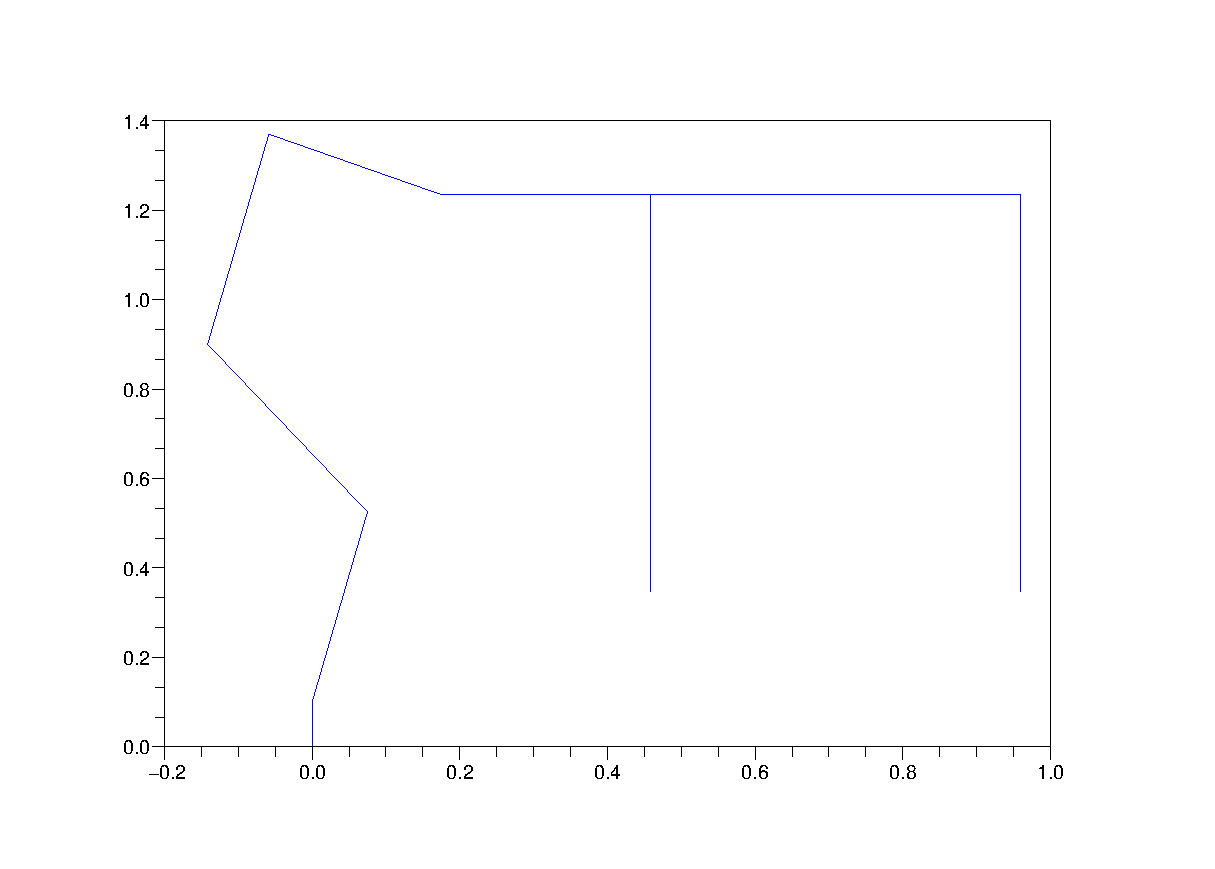
\includegraphics[width=0.8\columnwidth]{images/simu/positionInit.eps}
\caption{Position initiale du modèle}
\label{fig:positionInit}
\end{figure}



\subsubsection{Prise en compte des contraintes de pose du poignet}

Pour prendre en compte l'utilisation du déambulateur et donc les contraintes de hauteur et d'orientation du repère effecteur, on implémente une commande proportionnelle simple (en remplacement du modèle géométrique inverse). 

Soit $X$ la position courante de l'effecteur et $X^*$, sa position désirée, telles que $X=[x,\theta]$ et $X^*=[h,\theta ]$.
La tâche à réguler est 
\begin{align}
e1&=X^*-X
\end{align}

Le jacobien du robot est 
\begin{align}
J(q)&=[J_x(q) , J_y(q), J_{\theta}(q)]^T
\end{align} 

Le jacobien de la tâche est donc 
\begin{align}
J_1(q)&=[J_x(q) , J_{\theta}(q)]^T
\end{align}

D'où :
\begin{align}
		\dot q_1 &= -\lambda_1 J_1(q)e_1
\end{align}
\noindent avec $\lambda_1$ un scalaire positif.

\subsubsection{Prise en compte des limites articulaires}

On définit une tâche qui éloigne les positions articulaires de leurs butées (par exemple voir \cite{Chaumette01}).
La fonction de coût doit atteindre son maximum a proximité des butées (voir Fig. \ref{fig:butees}). \\

\begin{figure}[h]
\centering
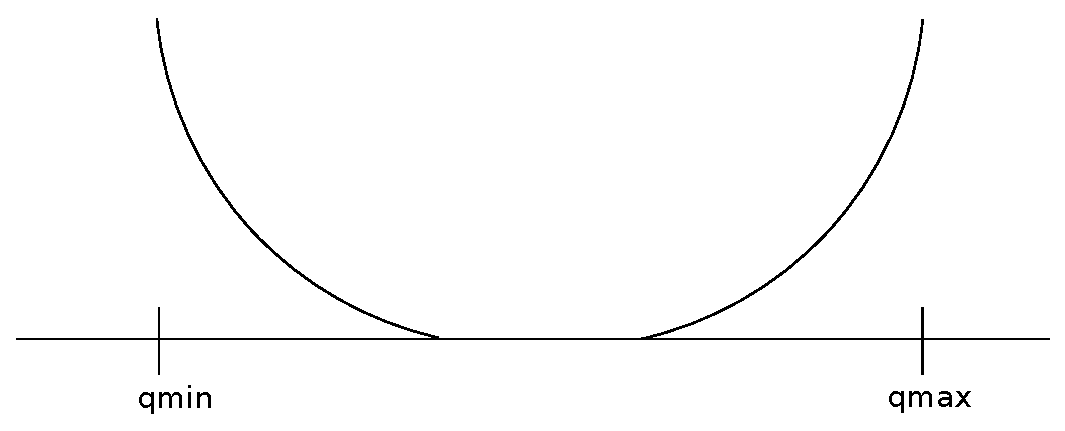
\includegraphics[width=0.5\columnwidth]{images/model/butees.eps}
\caption{Fonction de coût pour éloigner le système de ses butées.}
\label{fig:butees}
\end{figure}


On activera cette tâche uniquement pour les articulations proches des butées. Il y a deux manière de determiner cette condition. Soit $\delta q$, une marge de sécurité, soit $A$ et $B$ deux matrices $6\times6$ nulles,
\begin{itemize}
\item On peut tester $q_i$ et activer la commande si 
\begin{align}
q_i&<{q_i}_{min}+\Delta q
\end{align}
alors $A(i,i)=1$,  ou si 
 \begin{align}
 q_i&>{q_i}_{max}-\Delta q
\end{align}
alors  $B(i,i)=1$

\item Ou alors on peut tester $\dot{q}_i$ et activer la commande si 
\begin{align}
 \dot{q}_i  &<\frac{{q_i}_{min}-q_i}{\Delta t}
\end{align} 
alors $A(i,i)=1$,  ou si 
\begin{align}
\dot{q}_i  &>\frac{{q_i}_{max}-q_i}{\Delta t}
\end{align}
alors  $B(i,i)=1$
\end{itemize}

On peut alors écrire la fonction de coût sous la forme 

\begin{align}
e_2 = A\frac{q-q_{min}}{\Delta q} + B\frac{q-q_{max}}{\Delta q}
\end{align}


Le jacobien de cette tâche s'écrit 

\begin{align}
J_2 = A+B
\end{align}

\subsubsection{Prise en compte des deux tâches}
Pour réguler les deux tâches en tenant compte de la redondance du système, on peut écrire la fonction de coût sous la forme 
\begin{align}
e&=J_1^+e_1+P_1z
\end{align}
 \noindent où
 \begin{itemize}
 \item $e_1$ est la tâche principale à réaliser qui impose $m$ contraintes indépendantes sur les $n$ articulations du robot (avec $m<n$ )
 \item $e_2$ est une tâche secondaire. Seules les composantes de cette tâche qui n'enfreignent pas la tâche primaire peuvent être réalisées en utilisant la redondance du système.
 \item $J_1^+= J_1^T (J_1^T J_1)^-1$ est la pseudo inverse de Penrose et Moore.
 \item $P_1=I-J_1^+J_1$ est un opérateur de projection sur l'espace nulle de la tâche $e_1$
 \end{itemize}

On peut écrire
\begin{align}
\dot{q}&=J_1^+e_1+P_1z
\label{eq:Pz}
\end{align}
or
\begin{align}
J_2 \dot{q}&=e_2
\label{eq:dotq}
\end{align}

On introduit (\ref{eq:Pz}) dans (\ref{eq:dotq}) et on trouve l'expression de $z$: 
\begin{align}
J_2 (J_1^+e_1+P_1z)&=e_2\\
J_2  J_1^+e_1+ J_2P_1z&=e_2\\
z&= (J2P1)^+(e2-J_2J_1^+e_1)\\
\label{eq:z}
\end{align}

On introduit $z$ dans (\ref{eq:Pz}) et on obtient la loi de commande à deux tâches : 
\begin{align}
\dot{q}&=J_1^+e_1+P_1 (J_2P_1)^+(e2-J_2J_1^+e_1)
\label{eq:deuxtaches}
\end{align}

Or $P_1$ est nilpotent, donc on peut réécrire la loi de commande à deux tâche exacte (\ref{eq:deuxtaches})  :
\begin{align}
\dot{q}&=J_1^+e_1 + (J_2P_1)^+(e2-J_2J_1^+e_1)
\label{eq:deuxtachesfinal}
\end{align}

Dans certains papiers, on peut en trouver la version approchée qui permet d'obtenir une solution robuste : 
\begin{align}
\dot{q}&=J_1^+e_1 + P_1J_2^+e2
\label{eq:robuste}
\end{align}


Remarque, il est possible d'étendre le nombre de tâche à plus de deux tâches. Dans ce cas, le projecteur de la tâche $i$ peut s'écrire relativement à la tâche $i-1$ :

\begin{align}
\dot{q}_i &= \dot{q}_{i-1} + (J_iP_{i-1})^+(e_i-J_i\dot{q}_{i-1})\\
P_i&=P_{i-1}-(J_iP_{i-1})^+J_iP_{i-1}s
\end{align} 

En annexe \ref{annexe:algoActiveSet}, on trouve une autre implémentation possible de ces deux tâches en modélisant le problème sous la forme d'un problème quadratique simplifié. Il s'agit d'un QP "à un seul étage"qui permet de construire un "active set" de contraintes. Pour que l'implémentation soit compléte il manque la desactivation des contraintes en utilisant les multiplicateurs de Lagrange.

\subsubsection{Calcul d'une position respectant les contraintes}


Pour la simulation, on positionne le système dans une pose quelconque, par exemple $q_0=[10, -40, 40,110,-30,0]$ (voir figure \ref{fig:positionInit}). La position initiale apparait en bleu sur la figure. \\

En partant de cette position, on applique ensuite une loi de commande à deux tâches, telle que définie dans les sections précédentes. La tâche principale est la tâche d'évitement de butées que l'on veut absolument respecter. La tâche secondaire est la tâche de positionnement du poignet. L'utilisation du déambulateur contraint la hauteur du poignet ainsi que son orientation.\\

%Les codes sources sont dans les fichiers scilab src/control/controlHumanWalker.sci et  src/transformation/computeRobotModel.sci. Le code de test est main/testWalkerContraintes.sce. Il faut executer le script Load.sce pour charger les fonctions avant d'executer le script main/testWalkerContraintes.sce.\\


\begin{figure}[h]
\centering
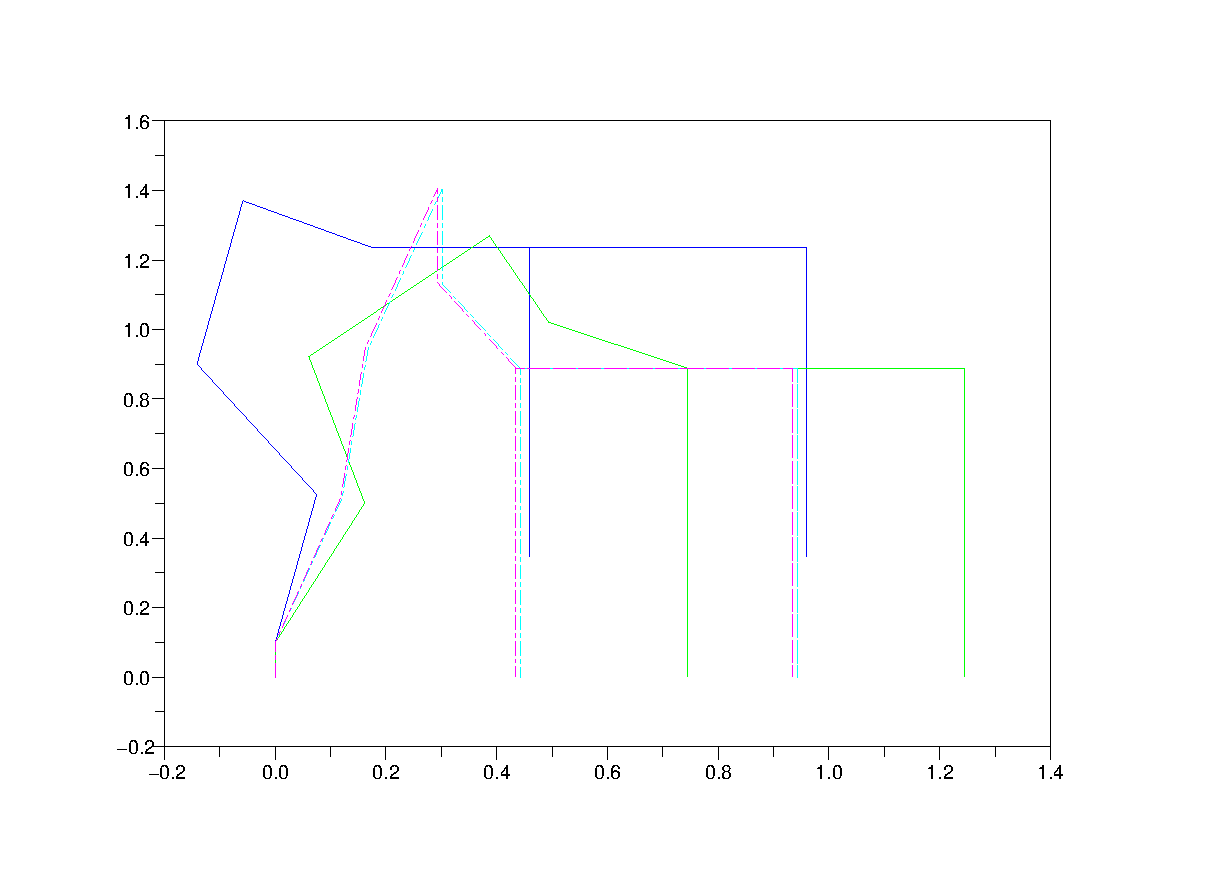
\includegraphics[width=0.8\columnwidth]{images/simu/applyConst.eps}
\caption{Calcul d'une position respectant les contraintes articulaires et les contraintes dues au déambulateur. En bleu, la position de départ, en vert la position obtenue sans prises en compte des contraintes articulaires. En magenta et en cyan, le résultat d'une loi de commande à deux tâches prenant en compte les contraintes articulaires et la hauteur du poignet.}
\label{fig:positionContrainte}
\end{figure}

\begin{figure}[h]
\centering
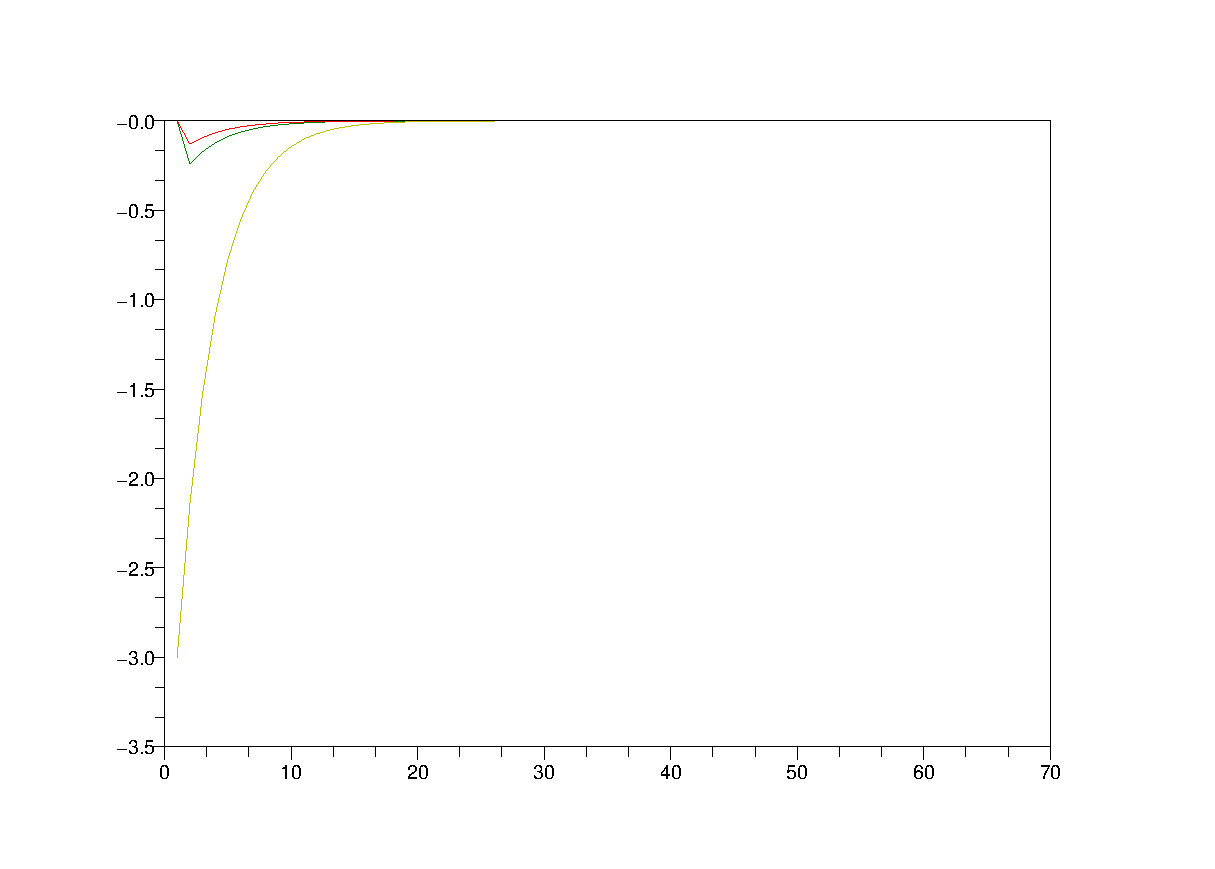
\includegraphics[width=0.8\columnwidth]{images/simu/erreurq1.eps}
\caption{Evolution de l'erreur de la tâche de positionnement}
\label{fig:erreur}
\end{figure}

La figure \ref{fig:positionContrainte} illustre le changement de posture du à la prise en compte des contraintes articulaires. La figure \ref{fig:erreur} montre l'évolution de l'erreur de la tâche de positionnement au fil du temps.
Pour que notre modèle soit complet, il faut maintenant générer une posture qui respecte les limites des couples articulaires.


\newpage
\section{Modélisation statique}

\subsection{Modélisation de l'humain}

\subsubsection{Position des centres d'inertie et masses des segments}

Les données sont extraites du livre de Allard et al. \cite{Allard11} (p60) et adaptée de \cite{Winter90}. La masse de chaque segment est donnée en pourcentage de la masse totale $m$ du sujet.
La figure \ref{fig:ModelHuman7forces} explicite la position des masses sur les différents segments. Pour le modèle sagital à 7 degrès de liberté, les masses des bras et des jambes sont doublées.

\begin{figure}[h]
\centering
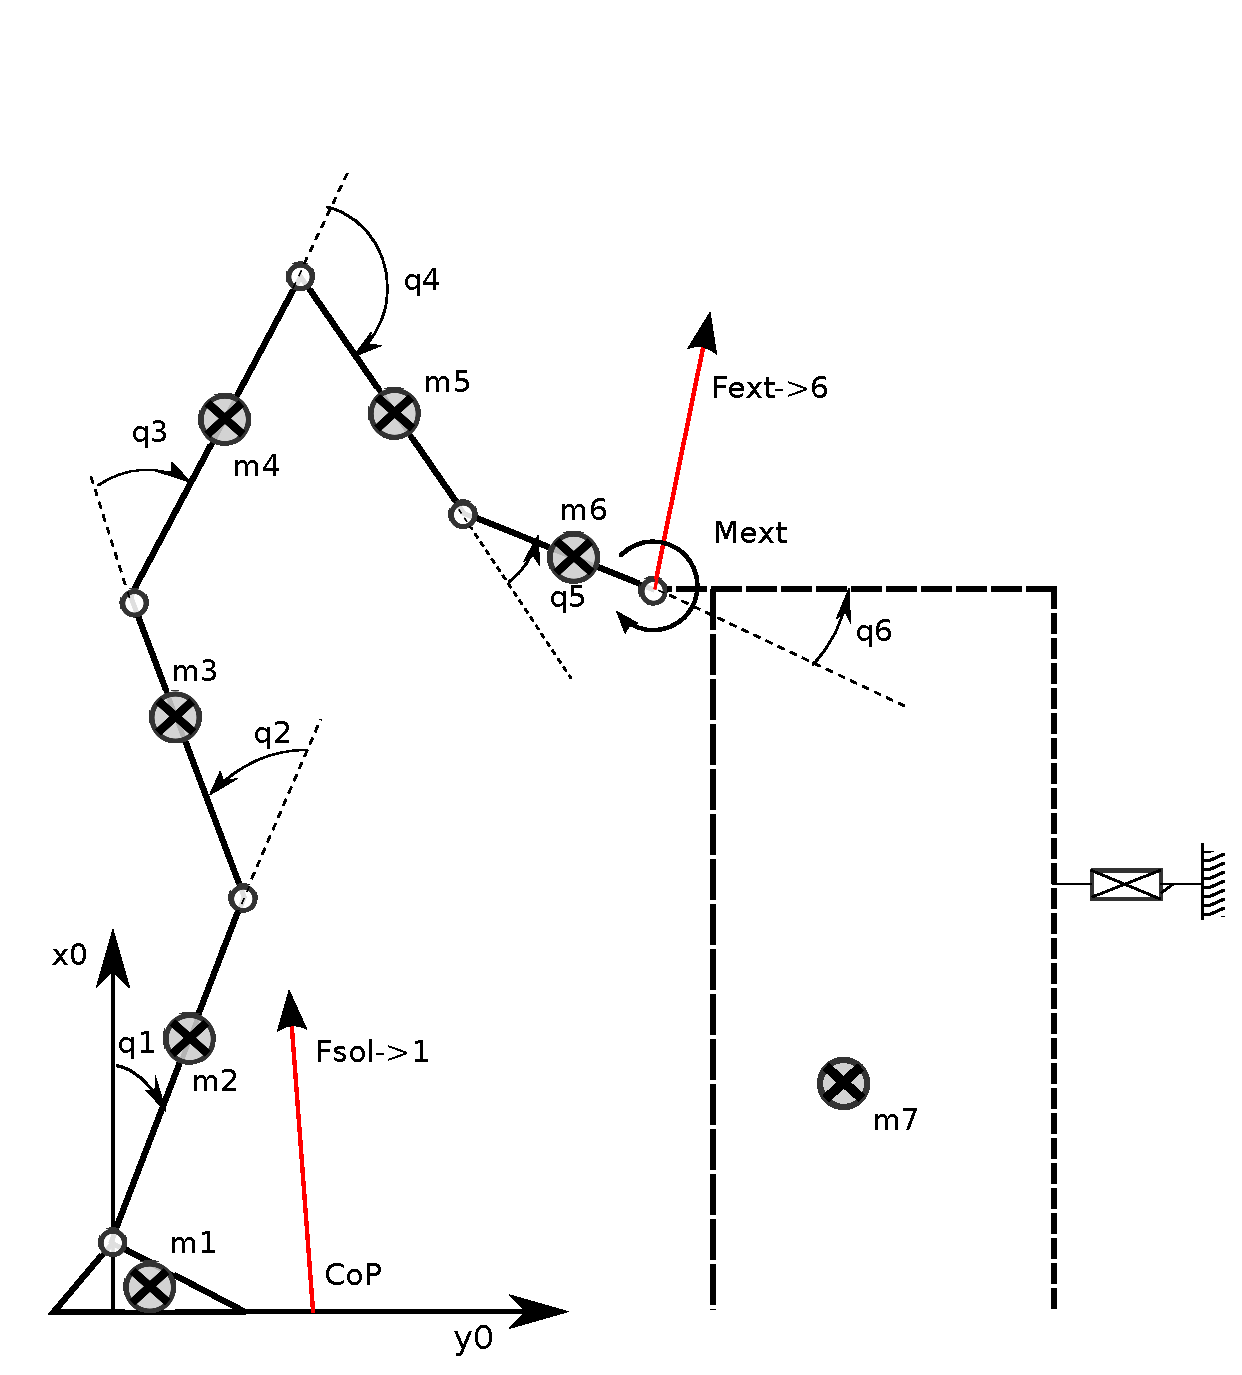
\includegraphics[width=0.5\columnwidth]{images/model/modeleHommeQ7.eps}
\caption{Modélisation du corps humain à 5 segments et 6 degrès de liberté. }
\label{fig:ModelHuman7forces}
\end{figure}

\begin{center}
\small{
\begin{tabular}{l |c |c| c| c| c| c|c}
membre & proxi. (\%)& dist.(\%) & rep. & $x$ & $y$ &  masses  & $m_i$\\
\hline
pied 	 			& 42.9 & 57.1 & $R_0$ & $ 0.429 \times 265 $		& 0 	& 0.0145 	&  $m_1=0.0145\times2\times m$\\
jambe 			& 43.3 & 56.7 & $R_1$ & $ 0.567 d_2$ 	& 0						& 0.0465 	&  $m_2= 0.0465\times2\times m$\\
cuisse 			& 43.3 & 56.7 & $R_2$ & $ 0.567 d_3$ 	& 0						& 0.1 			&   $m_3=0.1\times2\times m$\\
tronc et tête & 60.4 & 39.6 & $R_3$ & $ 0.396 d_4$ 	& 0						& 0.578 		&   $m_4=0.578\times m$\\
bras				& 43.6	& 56.4 & $R_4$ & $ 0.436 d_5$ 	& 0						& 0.028    	&  $m_5=0.028\times 2\times m$\\
avant-bras	& 43 	& 57		& $R_5$ & $0.43 d_6$		& 0						& 0.016 		& $m_6=0.016\times2\times m$
\end{tabular}}
\end{center}

\subsubsection{Calcul du centre de masse}

Le centre de masse est simplement le barycentre de tous les centres d'inertie :

\begin{align}
C=\sum_{i=1}^{6}{m_iC_i}
\end{align}

ou $C_i$ sont les centre de masse segmentaires et $m_i$ la masse du segment.

\subsubsection{Calcul de forces articulaires}

On considère que le système est statique. Pour chaque sous système, d'après le théorème fondamental de la dynamique on a donc :
\begin{align}
\sum_{i=1}^{6}F_i=0
\end{align}


\paragraph{modèle Human7}
On part d'une extrémité de la chaîne, par exemple, de  la force au poignet et on remonte de proche en proche pour trouver la force à chaque articulation (voir Fig. \ref{fig:propagationForce}).

Soit $F_{ext\rightarrow 6}$ la force exercée par le déambulateur sur le poignet. Connaissant le poids de l'avant bras  $F_{P\rightarrow 6}$, on en déduit alors simplement la force exercée par le bras sur l'avant bras au niveau du coude  $F_{5\rightarrow 6}$: 

\begin{align}
F_{5\rightarrow 6} = - F_{ext\rightarrow 6} -F_{P\rightarrow 6}
\end{align}
\begin{figure}[h]
\centering
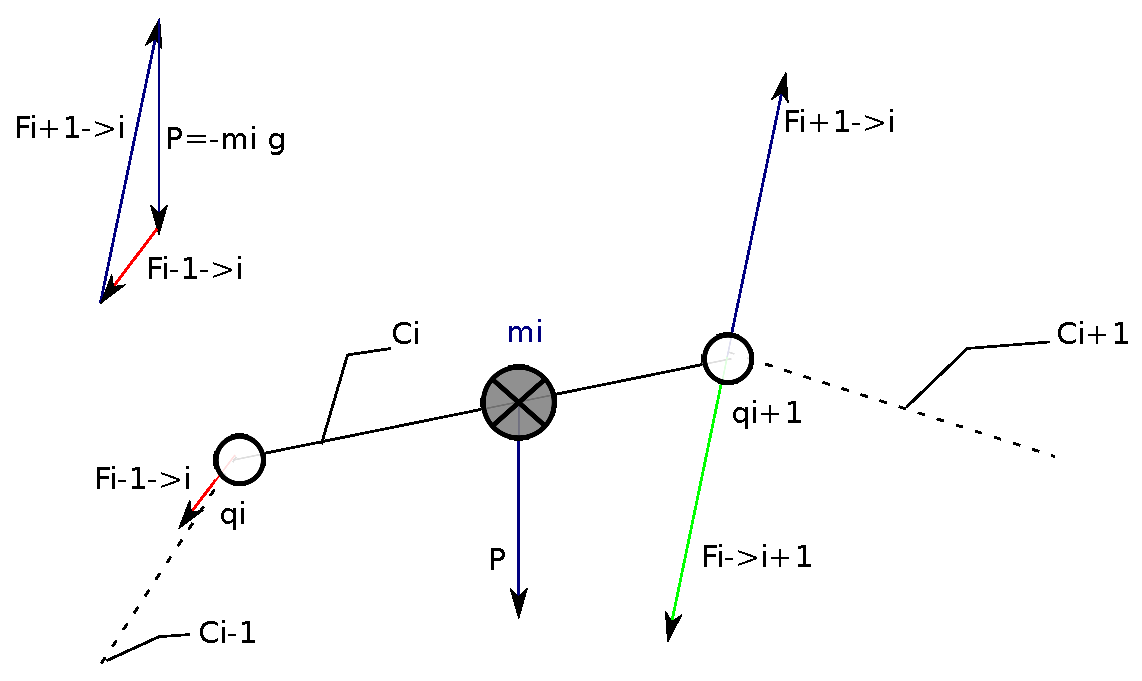
\includegraphics[width=0.8\columnwidth]{images/model/propagationForce.eps}
\caption{Propagation des forces d'une articulation à la précédente en utilisant l}
\label{fig:propagationForce}
\end{figure}

L'algorithme générique est le suivant : 
\begin{algorithm}[h]
\caption{Propagation des forces pour Human7}
\begin{algorithmic}[1]
\STATE $g \leftarrow 9.81$
\STATE $F_{i+1\rightarrow i} \leftarrow F_{ext\rightarrow 6}$
\STATE $F\leftarrow 0_{3\times6}$
\FOR {$i\leftarrow 6 $ \TO $i\leftarrow 0$}
	\STATE$F_{P_{i}\rightarrow i} \leftarrow \begin{bmatrix}-m_ig& 0& 0 \end{bmatrix}$
	\STATE$F_{i-1\rightarrow i} \leftarrow - F_{P_{i}\rightarrow i} -F_{i+1\rightarrow i} $
	\STATE $F_{i+1\rightarrow i}  \leftarrow -F_{i-1\rightarrow i}$
	\STATE $F[i] \leftarrow F_{i+1\rightarrow i}$
\ENDFOR
\RETURN $F$
\end{algorithmic}
\end{algorithm}


\paragraph{modèle Human4}

Pour le modèle Human4, seules 3 forces sont considérée : 
\begin{itemize}
\item La  force du déambulateur sur le poignet $F_{ext\rightarrow S}$
\item Le poids de la personne appliqué au centre d'inertie du tronc, tous les autres masses segmentaires étant négligées. $F_{P\rightarrow S}$
\item La force de réaction au sol $F_{0\rightarrow S}$.
\end{itemize}

En supposant qu'on connait la force au poignet, on peut calculer la résultante au sol.
\begin{align}
F_{0\rightarrow S} &= -F_{ext\rightarrow S}-F_{P\rightarrow S}
\end{align}



\subsubsection{Calcul des couples articulaires}

\paragraph{Modèle Human7}
On peut également propager les couples articulaires de proche en proche en partant de l'effecteur.
Le moment résultant des forces extérieures et du poids sur le coude s'écrit :

\begin{align}
\Gamma_5 = \Gamma_6+ 0_60_5\times F_{ext\rightarrow 6} + OI_6O_5\times  F_{P_6\rightarrow 6}
\end{align}

L'algorithme générique est le suivant : 
\begin{algorithm}[h]
\caption{Propagation des moments pour Human7}
\begin{algorithmic}[1]
\STATE $g \leftarrow 9.81$
\STATE $\Gamma_{i+1} \leftarrow \Gamma_{ext}$
\STATE $\Gamma\leftarrow 0_{3\times6}$
\FOR {$i\leftarrow 6 $ \TO $i\leftarrow 0$}
	\STATE $ci\leftarrow O_i-OI_i$
	\STATE $sl\leftarrow O_i-O_{i+1}$
	\STATE $\Gamma _i \leftarrow \Gamma _{i+1}+ci\times P[i]+sl\times F[i]$
	\STATE $\Gamma _{i+1}\leftarrow\Gamma _i$ 
	\STATE $\Gamma[i]\leftarrow\Gamma _i$
\ENDFOR
\RETURN $\Gamma$
\end{algorithmic}
\end{algorithm}

\paragraph{Modèle Human4}

Pour le modèle Human4, la calcul du couple est également très simple. Il suppose de connaitre la position du centre de masse du tronc et la position du poignet relativement aux pieds, la masse de la personne et la force et le couple exterieur.

On peut ainsi calculer le couple au niveau des pieds.
\begin{align}
\Gamma_0= \Gamma_{ext}+ 0_60_0\times F_{ext\rightarrow 6} + OI_4O_0\times  F_{P_4\rightarrow 4}
\end{align}


\subsubsection{Calcul du point de moment nul}

Un des critères de stabilité couramment utilisé est la position du ZMP, c'est à dire le point de moment zéro sur le plan du sol.

\paragraph{Pour le modèle Human7}
\begin{figure}[h]
\centering
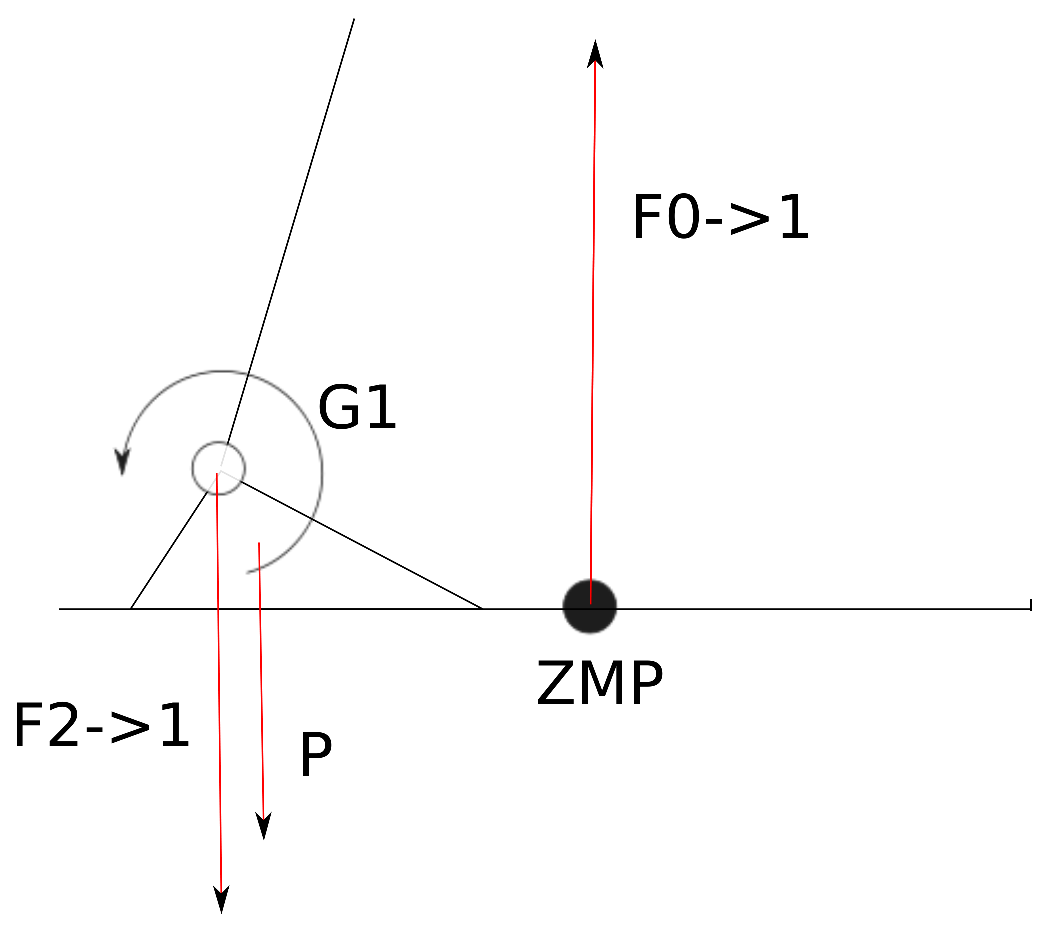
\includegraphics[width=0.5\columnwidth]{images/model/ZMPpied.eps}
\caption{Pour le modèle Human7, la position du ZMP dépend du couple exercé sur la cheville, des paramètres d'inertie du pied et de la force résultante}
\label{fig:ZMPpied}
\end{figure}

Pour ce modèle sagital, la position du ZMP a pour composantes $\begin{bmatrix} 0 &y_{ZMP}& 0\end{bmatrix}$.
On veut trouver $y_{ZMP}$ tel que le moment résultant au point $y_{ZMP}$ soit nul.

Soit 
\begin{itemize}
\item $\begin{bmatrix} x_{ci1} &y_{ci1}& z_{ci1}\end{bmatrix}y$ la position du centre d'inertie du pied 
\item $\begin{bmatrix} x_{2} &y_{2}& z_{2}\end{bmatrix}y$ la position du centre articulaire de la cheville
\item $\begin{bmatrix} -m_1g &0& 0\end{bmatrix}$ les trois composantes du poids du pied
\item $F_{2\rightarrow1}=\begin{bmatrix} F_x &F_y& F_z\end{bmatrix}$ les efforts appliqués à la cheville
\item $\Gamma_2=\begin{bmatrix} \Gamma_x &\Gamma_y& \Gamma_z\end{bmatrix}$ le couple appliqué à la cheville.
\end{itemize}

On obtient alors (voir détail en annexe \ref{annexe:ZMP})

\begin{align}
y_{ZMP}=\frac{m_1gy_{ci1}+F_yx_2-F_x y_2-\Gamma_z}{m_1g-F_x}
\label{eq:ZMP}
\end{align}


\paragraph{Pour le modèle Human4} 

Pour le modèle Human4, la formule est identique, sauf qu'on considère la force appliquée au poignet et son point d'appui au lieu d'utiliser la force appliquée à la cheville et le poids total au lieu d'utiliser uniquement le poids du pied. On trouve

Soit 
\begin{itemize}
\item $\begin{bmatrix} x_{ci4} &y_{ci4}& z_{ci4}\end{bmatrix}y$ la position du centre d'inertie du tronc
\item $\begin{bmatrix} x_{6} &y_{6}& z_{6}\end{bmatrix}y$ la position du centre articulaire du poignet
\item $\begin{bmatrix} -mg &0& 0\end{bmatrix}$ les trois composantes du poids total
\item $F_{2\rightarrow1}=\begin{bmatrix} F_{6x} &F_{6y}& F_{6z}\end{bmatrix}$ les efforts appliqués au poignet
\item $\Gamma_6=\begin{bmatrix} \Gamma_{6x} &\Gamma_{6y}& \Gamma_{6z}\end{bmatrix}$ le couple appliqué au poignet.
\end{itemize}
\begin{align}
y_{ZMP}=\frac{mgy_{ci4}+F_yx_6-F_x y_6-\Gamma_{6z}}{mg-F_x}
\label{eq:ZMP}
\end{align}


\subsubsection{Limites des couples et forces}

C'est sans doute sur ces aspects couples et forces max que le corps humain se différencie le plus d'une modélisations idéale robotique. En effet, ils varient selon la position articulaire et la direction du mouvement. 
Ainsi, pour une même articulation, il faut parler de couple max en extension, en flexion, en adduction, en abduction, etc... 
Pour schématiser grossièrement, le couple dépend de l'allongement des muscles flechisseur et extenseur. De la mêem manière, les forces max, varient selon la position articulaire, le sens d'execution du mouvement et la vitesse d'execution du mouvement. \\


Dans la littérature du domaine, les couples et les forces max sont donc caractérisés pour des positions précises du membres étudié et pour des gestes précis. La majorité des modèles sont conçus en conditions isométriques. Par exemple, Delp et al etudient les couples maximum pour le poignet dans des conditions isométriques \cite{delp1996}. D'autres études proposent de caractériser le bras dans des condition isocinétiques. Khalaf et al. \cite{Khalaf2001} propose une base de données normalisée acquise dans des conditions isocinétique. Ghallagher et al. \cite{gallagher1996,gallagher1997} etudie l'effet de l'age, du bras dominant et de la vitesse d'experimentation sur les couples max pour le coude et l'épaule. Ils montrent par exemple que l'âge impacte les capacité en flexion/extension mais pas en pronation/supination.


L'ordre de grandeur des couple max pour les articulations de notre modèle sagital est $100Nm$. On peut fixer cette valeur en première approximation. Il est possible d'affiner ce modèle en construisant une fonction qui le profil présenté sur la figure \ref{fig:profilcouple}. Le couple max varie en fonction de la position articulaire. Il atteint un premier sommet ou s'exprime le couple maximal des muscles. Il redescend ensuite jusqu'à un pallier, plus haut que le minimum de départ et remonte en un pic qui peut dépasser le maximum musculaire. Ce pique est le couple résistant des tendons et ligaments.

\begin{figure}[h]
\centering
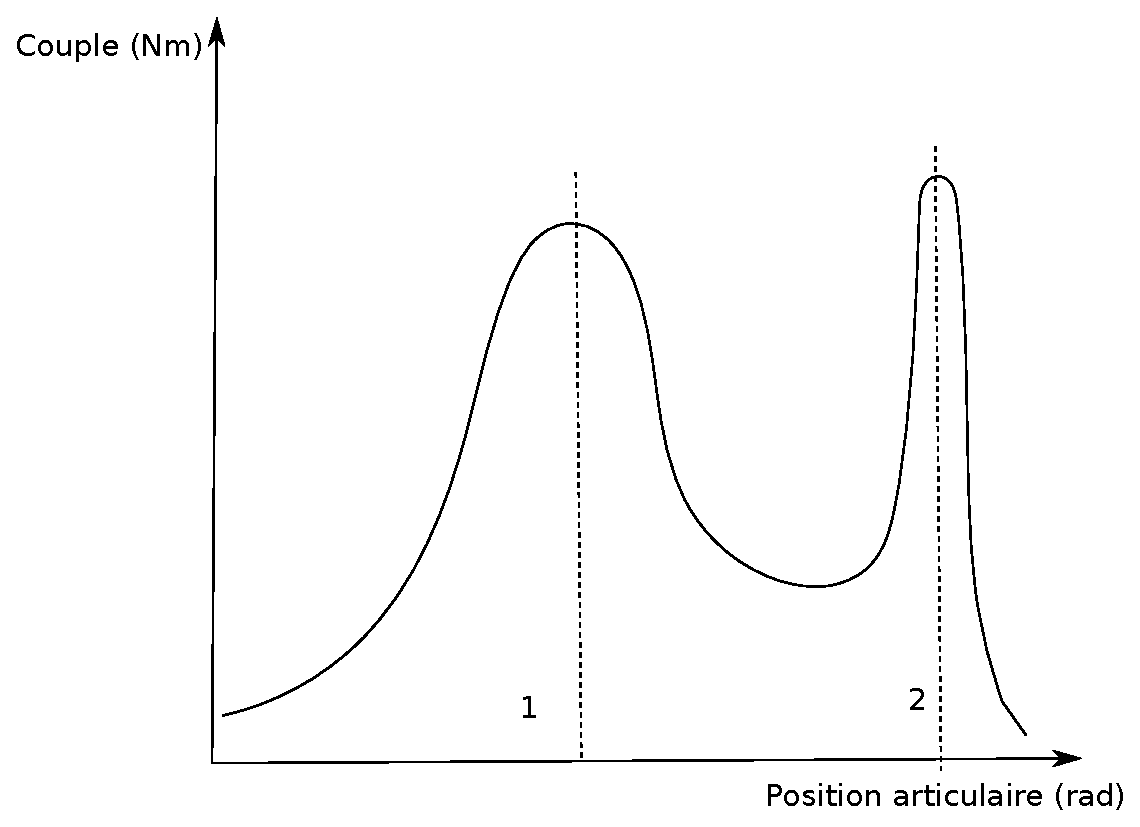
\includegraphics[width=0.5\columnwidth]{images/model/couples.eps}
\caption{Profil de l'évolution du couple en fonction de la position articulaire}
\label{fig:profilcouple}
\end{figure}


\subsection{Simulation}

\subsubsection{Absence d'appui sur la poignée }



Pour tester  la propagation des forces, on applique une force nulle sur la poignée. Le système a donc globalement deux forces : la réaction au sol et le poids. Si la propagation a fonctionné, pour une personne pesant 70 kg, on devrait trouver 
\begin{align}
F_{1\rightarrow 0}&=-mg\\
&=686.7Nm
\end{align}


On part d'une position quelconque $q_0=\begin{bmatrix}10& -40& 40& 110& -30& 0\end{bmatrix}$, on applique les contraintes géométriques dues à l'utilisation du déambulateur et les contraintes articulaire pour obtenir une position réaliste du système humain-deambulateur $q= \begin{bmatrix}7.0&-13.3&23.1&169.0&-30&-65.8\end{bmatrix}$ (voir Fig \ref{fig:positionContrainteF}). La masse totale de la personne est $m=70kg$.

 
 \begin{figure}[h]
\centering
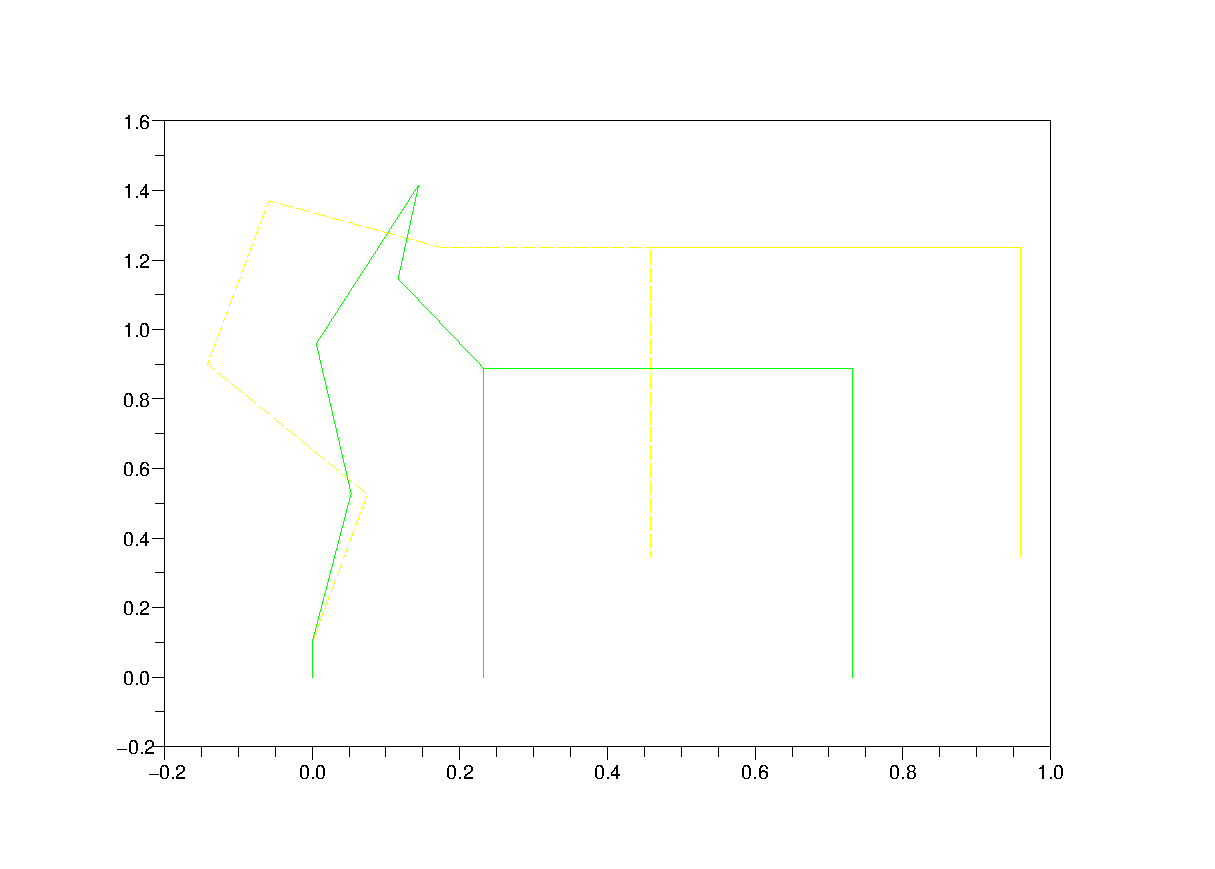
\includegraphics[width=0.8\columnwidth]{images/simu/Fext0/positionContrainte.eps}
\caption{Position sous contraintes géométriques.}% Les ronds rouges représentent les positions des centres d'inertie.}
\label{fig:positionContrainteF}
\end{figure}

Connaissant la position $q$ et les position des centres d'inertie segmentaire, on peut calcule le COM et sa projection (voir Fig. \ref{fig:COM} ).

 \begin{figure}[h]
\centering
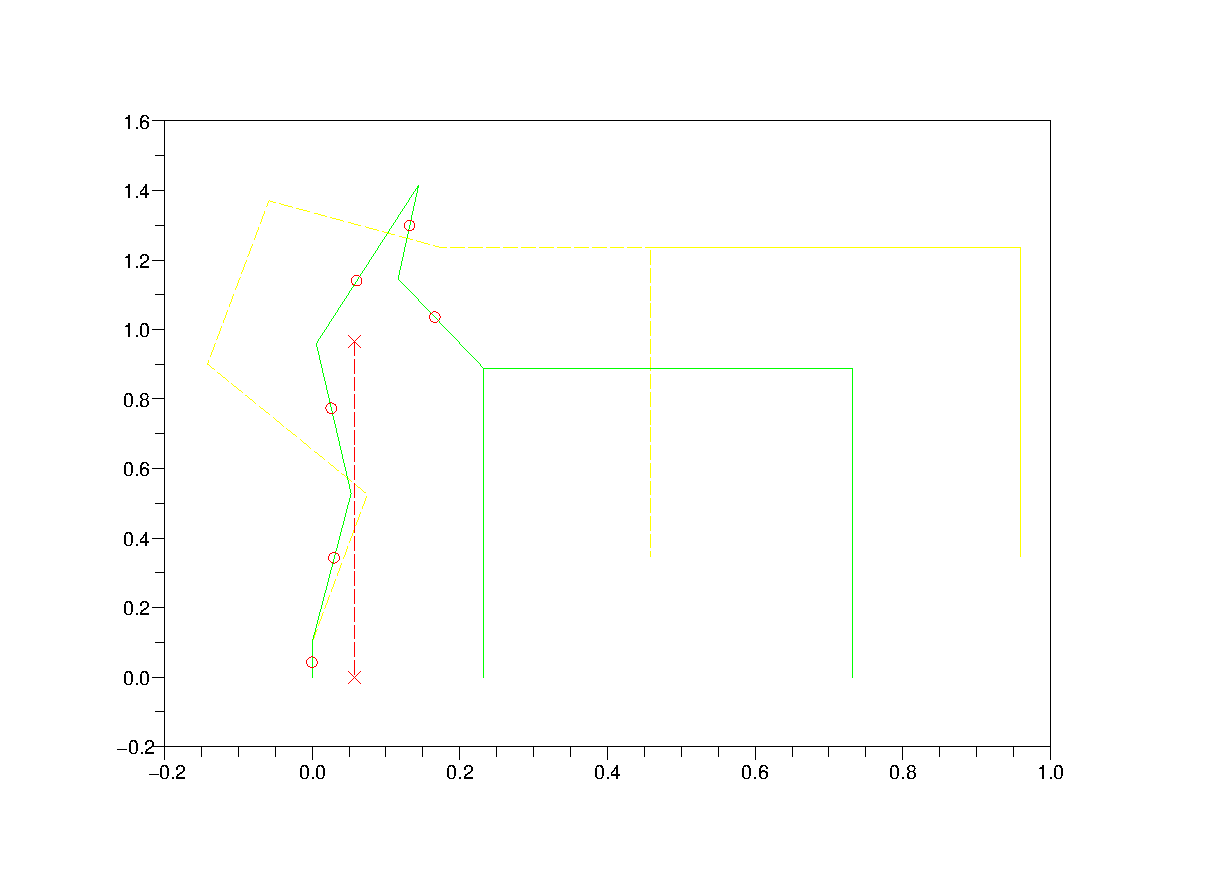
\includegraphics[width=0.8\columnwidth]{images/simu/Fext0/COM.eps}
\caption{Les ronds rouges représentent les positions des centres d'inertie segmentaire, la croix rouge représente le centre de masse équivalent et sa projection sur le sol.}
\label{fig:COM}
\end{figure}

On utilise la formule de propagation des forces pour évaluer la force de réaction au sol lorsqu'aucune force ne s'applique sur le poignet. On trouve bien $F_{1\rightarrow 0}=686.7Nm$ (voir fig \ref{fig:Fext0}).

 \begin{figure}[h]
\centering
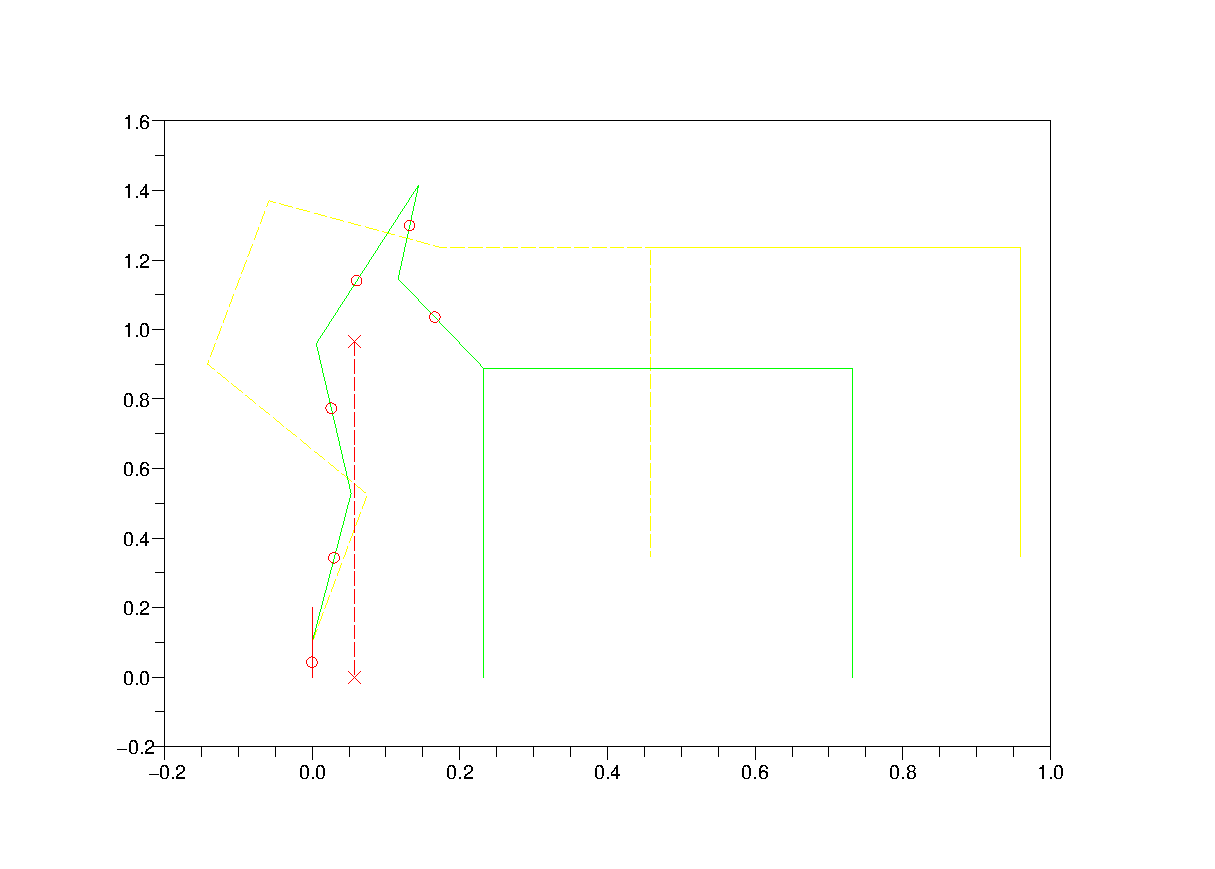
\includegraphics[width=0.8\columnwidth]{images/simu/Fext0/Fext0.eps}
\caption{Représentation des forces extérieures appliquées sur le système. La force exercée par le déambulateur sur le poignet est nulle. On retrouve bien la force de réaction au sol égale à $mg$.}
\label{fig:Fext0}
\end{figure}

On calcule ensuite la position du ZMP en utilisant l'equation \ref{eq:ZMP}. La figure \ref{fig:ZMP} montre que la position obtenue coincide exactement avec la position de la projection du centre de masse, dans ce cas sans appui. La position du ZMP est $57mm$ à l'avant des pieds.

Si on utilise le modèle Human4, on trouve un ZMP à $60mm$ à l'avant des pieds du sujet. L'approximation est donc judicieuse pour cette position $q$ (voir figure \ref{fig:ZMPHu4_0}). 

 \begin{figure}[h]
\centering
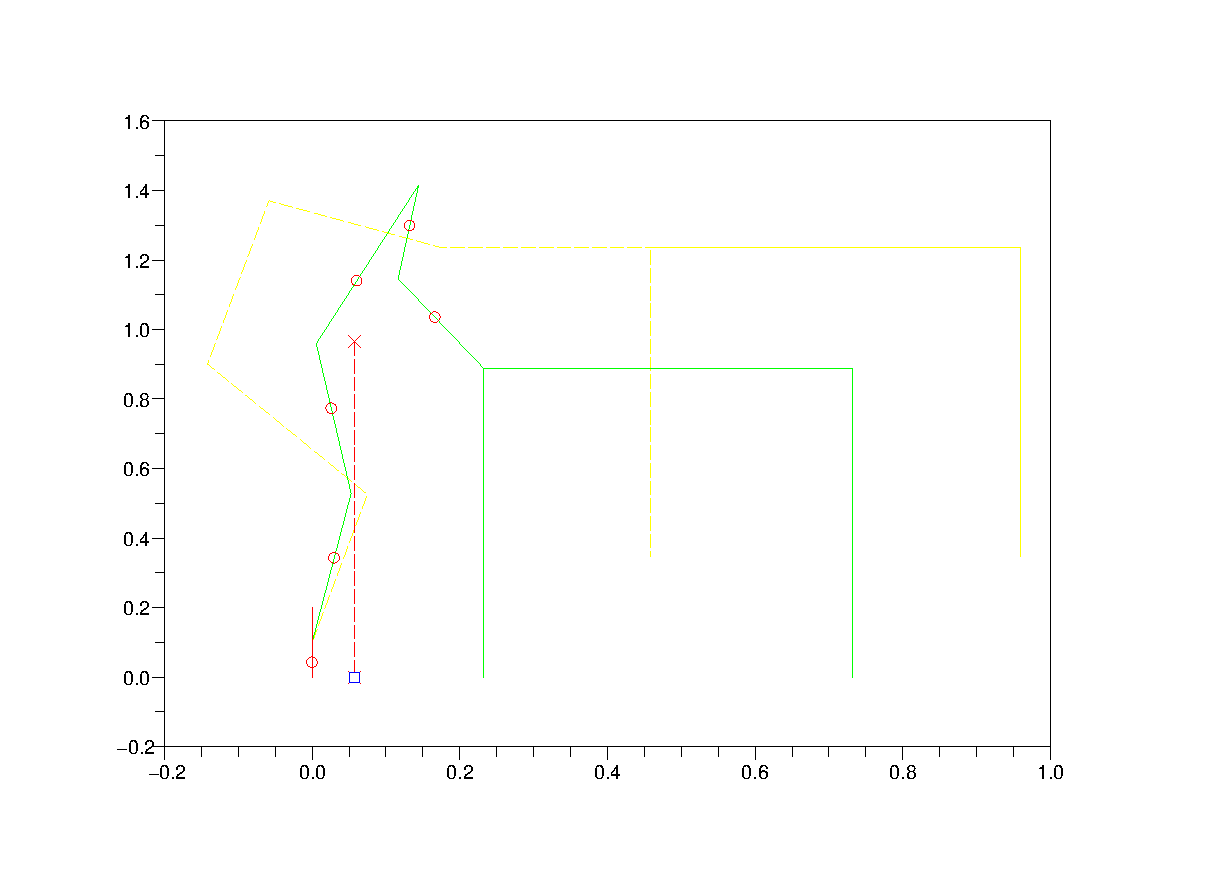
\includegraphics[width=0.8\columnwidth]{images/simu/Fext0/ZMP.eps}
\caption{Le carré bleu représente la position du ZMP. Dans le cas ou le système n'est pas en appui sur le déambulateur, le ZMP est confondu avec la projection du centre de masse.}
\label{fig:ZMP}
\end{figure}

 \begin{figure}[h]
\centering
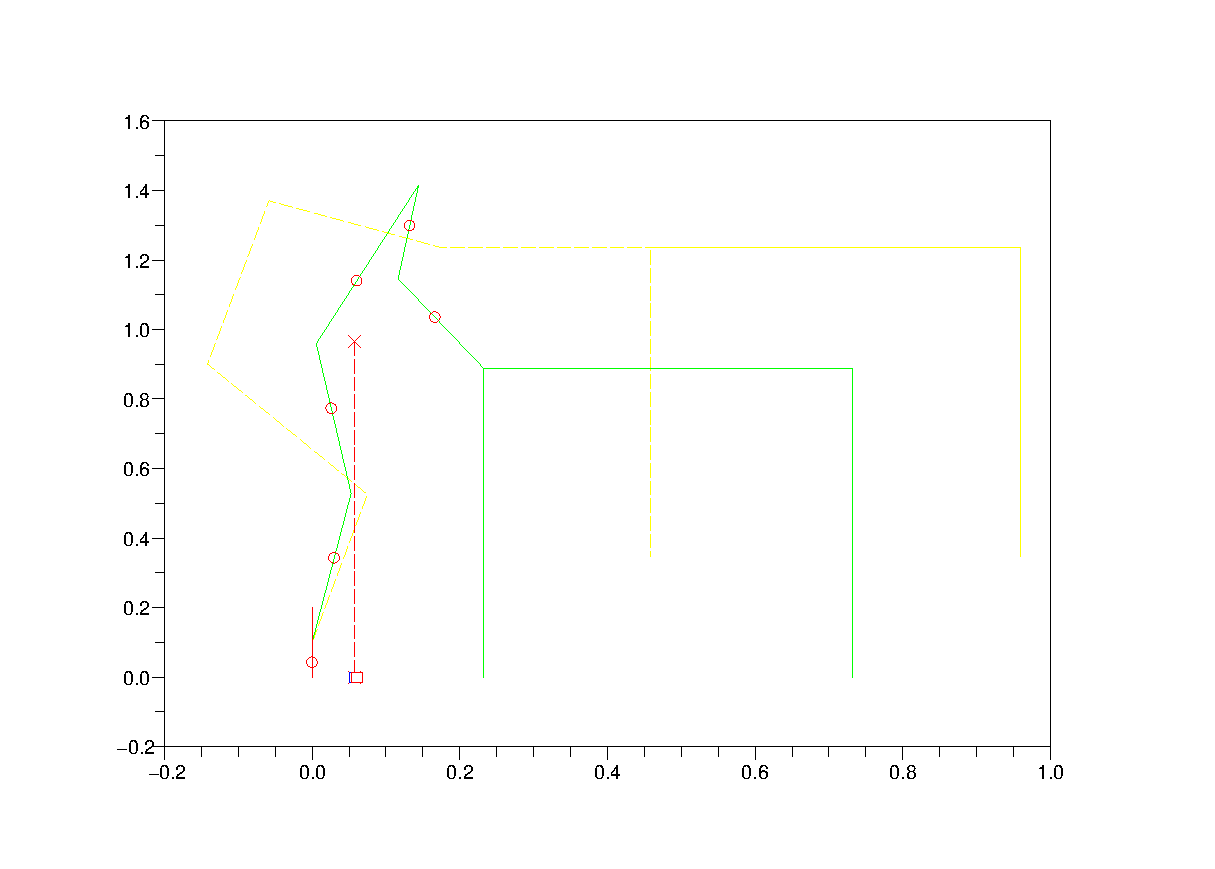
\includegraphics[width=0.8\columnwidth]{images/simu/Fext0/ZMPHu4.eps}
\caption{Le carré rouge représente la position du ZMP pour el modèle Human4. }
\label{fig:ZMPHu4_0}
\end{figure}

Dans cette simulation, on estime les couples suivants : 
\begin{align}
\Gamma & = 
	\begin{bmatrix}
		0&0&0&0&0&0\\
		0&0&0&0&0&0\\
		-39.63&-39.63&-5.83&-31.5&-0.21&-1.5&0
	\end{bmatrix}
\end{align}

\noindent et les forces suivantes :
\begin{align}
F & = 
	\begin{bmatrix}
	    -686.7&-666.8&-602.9&-465.6.5&-68.7&-30.2&0\\
		0&0&0&0&0&0\\
		0&0&0&0&0&0
	\end{bmatrix}
\end{align}


\subsubsection{On applique une force de 100 Nm sur la poignée }

On part des mêmes conditions initiales que l'expérience précédente, mais on applique un couple de $100Nm$ sur la poignée. La figure \ref{fig:ZMP100Nm} montre la position du ZMP obtenu en bleu. Le ZMP recul vers les pieds du sujet, il se situe à $28mm$. Il n'est plus confondu avec le COM. Si on considère seulement le sujet, plus le ZMP est entre ses pieds, plus il est stable. Mathématiquement, on pourrait donc stabiliser la personne en augmentant cette force d'appui F. On peut aussi ramener le ZMP au milieu des pieds en modifiant la position du déambulateur.

Le ZMP approximé pour le modèle Human 4 se trouve à $31mm$ à l'avant du pied (voir figure \ref{fig:ZMPHu4100}). L'erreur d'approximation est plus conséquente que dans le cas ou la force est nulle mais reste raisonable. On pourrait utiliser cette approximation pour la commande. L'avantage est que cette écriture du ZMP dépend directement de la position de l'effecteur, de la force et du couple exterieure par l'équation (\ref{eq:ZMP}). Il est également possible d'obtenir le ZMP en fonction de ces paramètres pour la version Human7, avec une équation qui tiendra compte de toutes les positions des centres articulaires et de leurs masses. 

 \begin{figure}[h]
\centering
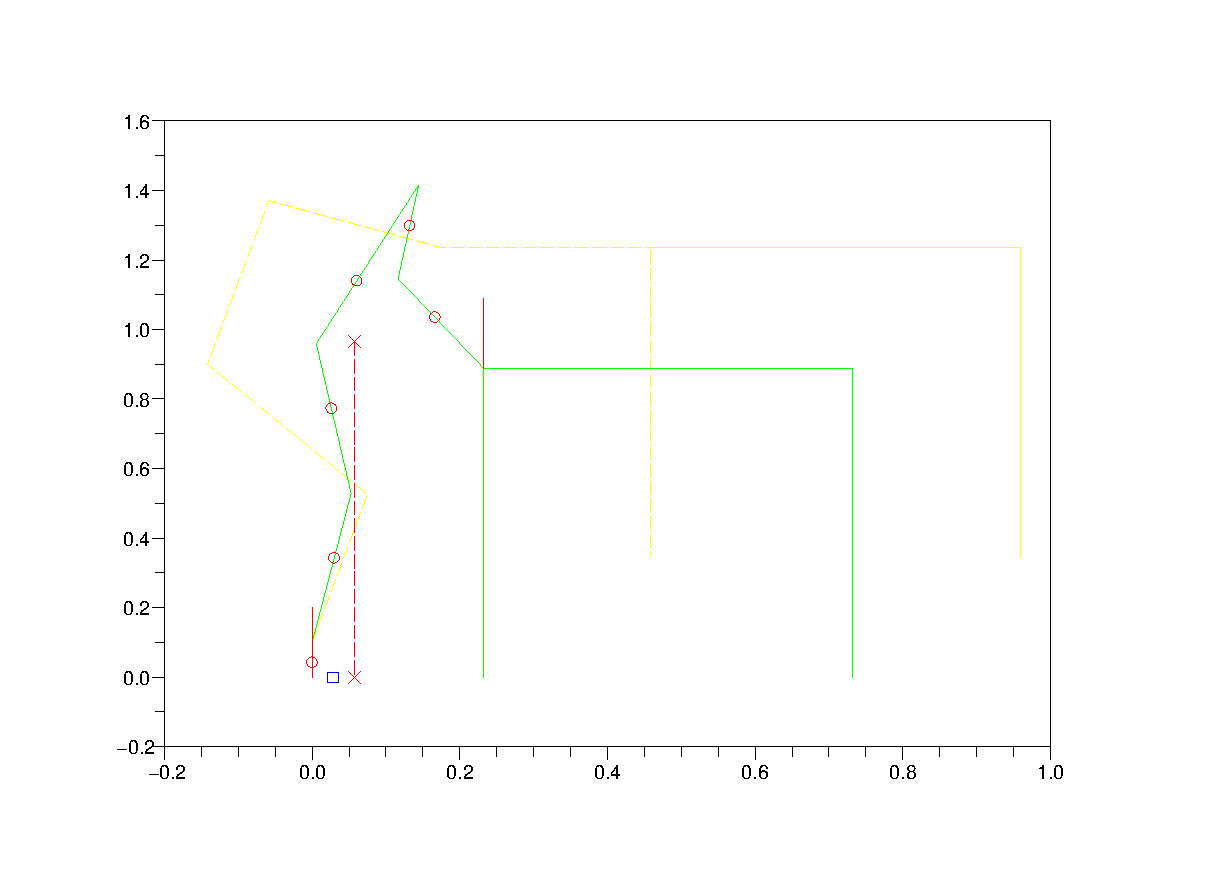
\includegraphics[width=0.8\columnwidth]{images/simu/Fext100/ZMP.eps}
\caption{Position du ZMP lorsque le sujet s'appui sur le déambulateur.}
\label{fig:ZMP100Nm}
\end{figure}

 \begin{figure}[h]
\centering
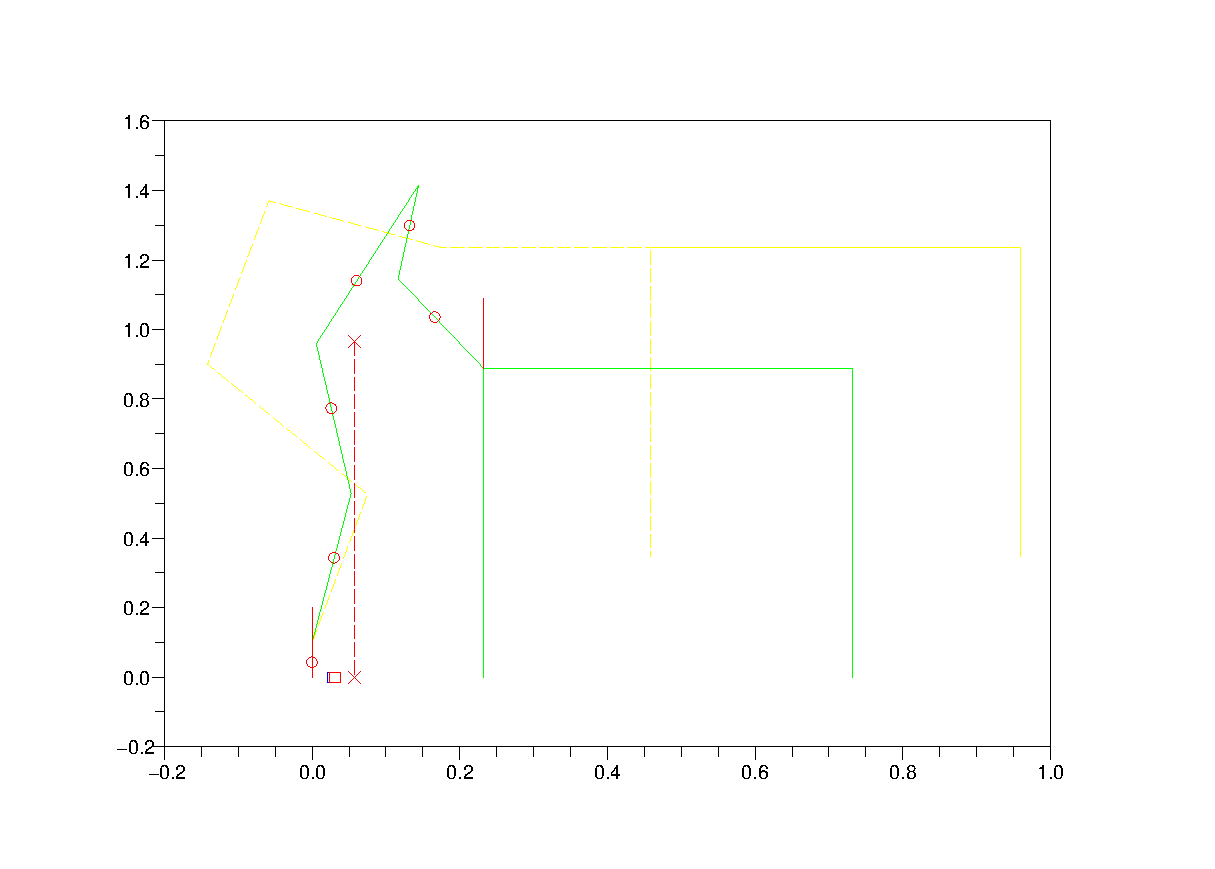
\includegraphics[width=0.8\columnwidth]{images/simu/Fext100/ZMPHu4.eps}
\caption{Le carré rouge représente la position du ZMP estimé pour le modèle Human 4}
\label{fig:ZMPHu4100}
\end{figure}

Dans cette simulation, on estime les couples suivants : 
\begin{align}
\Gamma & = 
	\begin{bmatrix}
		0&0&0&0&0&0\\
		0&0&0&0&0&0\\
		-16.39&-16.39&12.12&-8.81&8.61&10.1&0
	\end{bmatrix}
\end{align}

\noindent et les forces suivantes :
\begin{align}
F & = 
	\begin{bmatrix}
	    -586.7&-566.8&-502.9&-365.6.5&31.33&69.7&100\\
		0&0&0&0&0&0\\
		0&0&0&0&0&0
	\end{bmatrix}
\end{align}

\section{Loi de commande}

Pour assurer la stabilité du système, on peut écrire une loi de commande qui régule  la position du ZMP vers une position désirée tout en minimisant les couples articulaires: 
\begin{align}
ZMP&\rightarrow ZMP^*\\
\sum_i \alpha_i \Gamma &\rightarrow 0\\
q_i&<q_max
q_i&>q_min
x_6 \rightarrow h
\theta_{z6} \rightarrow \pi/2
\end{align}

\section{Perpectives}

\subsection{Rédiger la partie biblio sur l'équilibre}

La partie bibliographie sur l'équilibre est à inclure dans ce rapport.

\subsection{Validation du modéle sans appui}
En utilisant une plateforme de force et un systeme de motion capture, on peut vérifier que le calcul du ZMP ne soit pas trop faux en comparant le résultat à la position du centre de pression donné par la plateforme.

Il faut tester le modèle pour différentes positions. 

\subsection{Validation du modéle avec appui}

Pour valider le modèle avec appui, il faut se placer dans le même schéma mais disposer de capteurs de forces pour pouvoir évaluer la force sur les poignées.

En utilisant le motion capture et une plateforme de force, on doit pouvoir évaluer les paramètres $d$ et le centre de masse du tronc du modèle simple. Voire ... en utilisant la kinect a la place du motion capture. On a juste besoin de la position des pied relativement aux mains ce qu'on a avec le deambulateur equipe d'une kinect. Attention, en l'absence d'appui, on pourra juste trouver le $y$ du centre de masse .... 

\subsection{Vérifier le critère de stabilité}

Quel est le $ZMP^* $ pour que le système soit le plus stable possible ?

\subsection {Tester le ZMP pour tout un ensemble de position}

Ce test a déjà été fait, il ne reste plus qu'à l'écrire dans ce rapport.


\subsection{Développement de la loi de commande}

Il reste à écrire la loi de commande en fonction de $q$ et $\dot{q}$ et à l'intégrer a une commande multi tâche à trois niveau.

A priori, la commande se fera en modifiant la position du poignet, ie en deplacant le déambulateur et non pas en modifiant la force appliquée au niveau des poignées. Ce changement de position va nécessairement induire un changement de la force exercée qui va elle aussi impactée la position du ZMP. Il faudra tenir compte de ce paramètre.

Enfin, est ce qu'une telle commande permet encore à la personne d'avancer ou la contraint à rester sur place ? 
Plutot qu'un $ZMP^*$ il faut sans doute plutot proposer une trajectoire  $ZMP^*(t)$ qui anticipe la marche de la personne.\\
Cette version sera d'autant plus interessante dans des pentes.

\subsection{Augmenter le modéle}

Ajouter une seconde jambe et passer à un modéle marcheur et faire l'étude de la stabilité en cours de marche. Puis passer au modéle 3D.

Nous avons aussi fait de nombreuses hypothèses sur le modéle (sol plan, etc.) il faudra lever ces hypothèse.

\subsection{Estimation des paramètres en ligne}

Si le modèle Human 4 est suffisant, alors, nous n'avons besoin de connaitre que la position des pieds, la position du centre de masse et la force.

\subsection{Condition de stabilité du déambulateur}

Ajouter une contrainte sur les conditions de stabilité du déambulateur : il ne peut pas être soumis à n'importe quelle force au niveau des poignet sans se renverser.

\newpage
\appendix
\section{Modèle géométrique du modèle Human 7 }
\label{Annexe1}

La figure \ref{fig:ModelHuman7GMannexe} présente le modéle géométrique du système dans le plan sagital.

\begin{figure}[h]
\centering
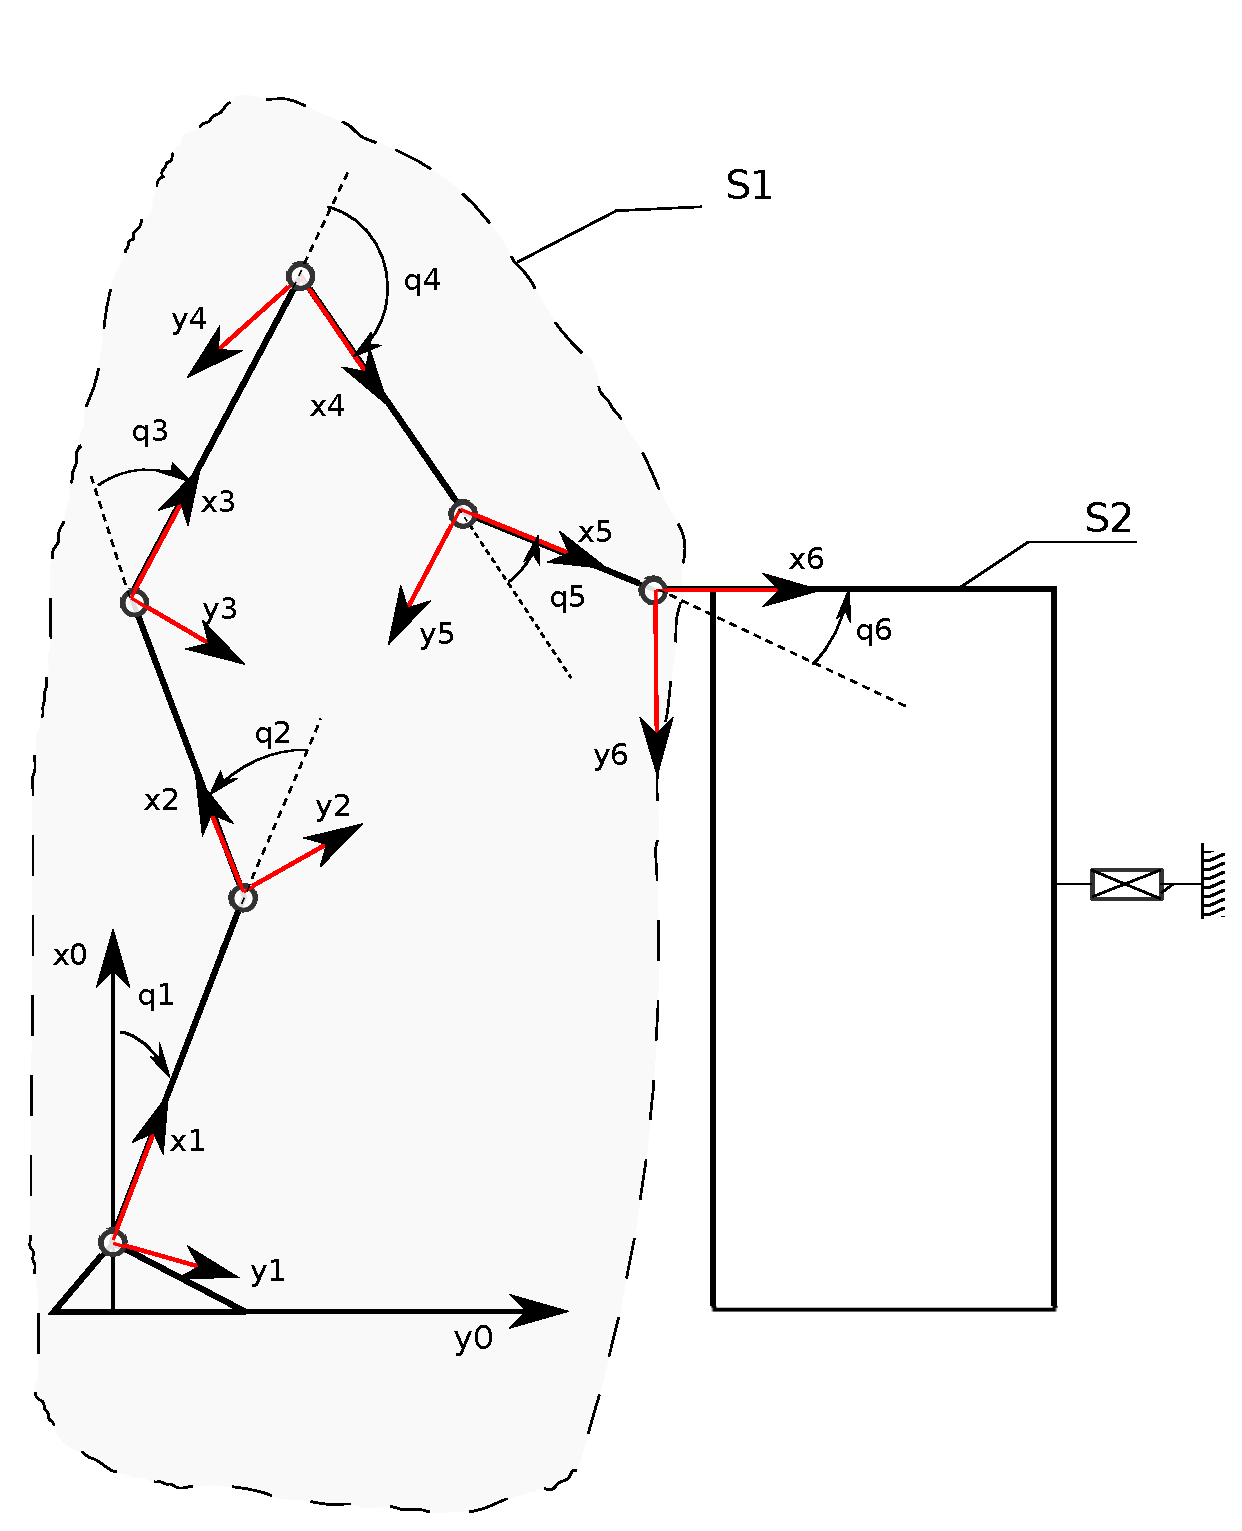
\includegraphics[width=0.5\columnwidth]{images/model/modeleHommeQ7MG.eps}
\caption{Modélisation géométrique du corps humain à 5 segments et 6 degrès de liberté.}
\label{fig:ModelHuman7GMannexe}
\end{figure}

\paragraph{Positionnement des repères} : nous utilisons la notation  de Khalil et Kleinfinger \cite{Khalil86a}. On note le repère $R_j$, le repère attaché au corps $j$ et la variable de l'articulation $j$ est notée $q_j$.

Le repère $R_j$ est défini de sorte que 
\begin{itemize}
\item l'axe $z_j$ est porté par l'axe de l'articulation $j$ ; 
\item l'axe $x_j$ est porté par la perpendiculaire commune à $z_j$ et $z_{j+1}$;
\end{itemize}

Le passage du repère $R_{j-1}$ au repère $R_j$ s'exprime en fonction de 4 paramètres : 
\begin{itemize}
\item $\alpha_j$ : angle entre les axes $z_{j-1}$ et $z_{j}$ correspondant à une rotation autour de $x_{j-1}$, toujours nul pour notre modèle sagital ;
\item $d_j$ : distance entre les axes $z_{j-1}$ et $z_{j}$ le long de l'axe $x_{j-1}$, ici, la longueur des segments \cite{Winter90};
\item $\theta_j$ : angle entre les axes $x_{j-1}$ et $x_{j}$ correspondant à une rotation autour de $z_j$, ici, ce sont directement les $q_i$;
\item $r_j$: distance entre $x_{j-1}$ et $x_{j}$ le long de $z_j$, toujours nul pour le modèle considéré.
\end{itemize}

Le tableau de paramètres pour le modèle à 7 degrès de liberté est : 

\begin{center}
\begin{tabular}{l c c c c}
$j$ & $\alpha_j$ & $d_j$ & $\theta_j$ & $r_j$\\
1 & 0 & 0.05 &$q_1$ & 0 \\
2 & 0 & 0.432 &$q_2$ & 0 \\
3 & 0 & 0.433 &$q_3$ & 0 \\
4 & 0 & 0.477 &$q_4$ & 0 \\
5 & 0 & 0.271 &$q_5$ & 0 \\
6 & 0 & 0.283 &$q_6$ & 0 
\end{tabular}
\end{center}


\paragraph{Matrices de transfert}
On se trouve dans un cas très simple ou tous changement de repere se font en effectuant une rotation en $z$ et une translation en $x$. Les changements de repères s'écrivent donc de manière très simple :

\begin{equation}
^{j-1}M_j =\begin{bmatrix}
							cos(\theta_j) & -sin(\theta_j) & 0 & d_j \\
							sin(\theta_j) & cos(\theta_j) & 0 & 0 \\
							0 & 0 & 1 & 0 \\
							0 & 0 & 0 & 1 \\
					\end{bmatrix}
\label{eq:changementRepere}
\end{equation} 

Par ailleurs, comme tous les axes articulaires sont parallèles, on peut écrire
\begin{equation}
^{0}M_j =\begin{bmatrix}
							\cos(\sum_{i=1}^j q_i) & -\sin(\sum_{i=1}^j q_i) & 0 & x_j \\
							\sin(\sum_{i=1}^j q_i) & \cos(\sum_{i=1}^j q_i) & 0 & y_j \\
							0 & 0 & 1 & 0 \\
							0 & 0 & 0 & 1 \\
					\end{bmatrix}
\label{eq:changementRepereDirect}
\end{equation} 

\noindent avec 
\begin{align}
	x_j &= d_1 + \sum_{i=2}^j d_i \cos( \sum_{k=1}^ {i-1}q_i) \\
	y_j &=  \sum_{i=2}^j d_i \sin( \sum_{k=1}^ {i-1}q_i)
	\label{eq:translation}
\end{align}

\section{Modèle cinématique du modéle Human 7}
\label{Annexe2}

Soit $^0X=(x,y,\theta)$ la position de l'effecteur dans le repère de référence $R_0$.  La jacobienne du modèle plan à 7 ddl est définie ainsi : 

\begin{equation}
dX = J(q) dq
\end{equation}

On peut l'obtenir par dérivation du modèle géométrique (voir \ref{Annexe2}). 
\begin{equation}
J_{ij} = \frac{\partial f_i}{\partial q_j}
\end{equation}

Comme toutes les articulations ont des axes parallèles, On peut écrire très simplement $\theta$
\begin{equation}
\theta =\sum_{i=1}^6 q_i 
\end{equation}
Et donc pour tout $i$ sa dérivée partielle selon $q_i$, est : 
\begin{equation}
\frac{\partial\theta}{\partial q_i} =1
\end{equation}

Pour la position dans le plan $(x_0,y_0)$, il suffit de dériver les expressions de $T_x$ et $T_y$ de l'équation (\ref{eq:translation}) :

\small{
\begin{align}
	\frac{\partial x_6}{\partial q_1} &=\!-d_2\sin q_1\! - \!d_3\sin (q_1+q_2)\! -\! d_4\sin (q_1+q_2+q_3)\! -\! d_5\sin (q_1+q_2+q_3+q_4)\!-\! d_6\sin (q_1 \!+ \! q_2 \! + \! q_3 \! +\! q_4\! +\! q_5)\\
	\frac{\partial x_6}{\partial q_2} &=-d_3\sin (q_1+q_2) - d_4\sin (q_1+q_2+q_3) - d_5\sin (q_1+q_2+q_3+q_4)- d_6\sin (q_1+q_2+q_3+q_4+q_5)\\
	\frac{\partial x_6}{\partial q_3} &=- d_4\sin (q_1+q_2+q_3) - d_5\sin (q_1+q_2+q_3+q_4)- d_6\sin (q_1+q_2+q_3+q_4+q_5)\\
	\frac{\partial x_6}{\partial q_4} &=- d_5\sin (q_1+q_2+q_3+q_4)- d_6\sin (q_1+q_2+q_3+q_4+q_5)\\
	\frac{\partial x_6}{\partial q_5} &=- d_6\sin (q_1+q_2+q_3+q_4+q_5)\\
	\frac{\partial x_6}{\partial q_6} &=0
	\label{eq:Jx}
\end{align}}

et
\small{
\begin{align}
	\frac{\partial y_6}{\partial q_1} &=d_2\cos q_1 + d_3\cos (q_1+q_2) + d4\cos (q_1+q_2+q_3) + d5\cos (q_1+q_2+q_3+q_4)+ d6\cos (q_1+q_2+q_3+q_4+q_5)\\
	\frac{\partial y_6}{\partial q_2} &= d_3\cos (q_1+q_2) + d_4\cos (q_1+q_2+q_3) + d_5\cos (q_1+q_2+q_3+q_4)+ d_6\cos (q_1+q_2+q_3+q_4+q_5)\\
	\frac{\partial y_6}{\partial q_3} &=d_4\cos (q_1+q_2+q_3) + d5\cos (q_1+q_2+q_3+q_4)+ d_6\cos (q_1+q_2+q_3+q_4+q_5)\\
	\frac{\partial y_6}{\partial q_4} &=d_5\cos (q_1+q_2+q_3+q_4)+ d_6\cos (q_1+q_2+q_3+q_4+q_5)\\
	\frac{\partial y_6}{\partial q_5} &=d_6\cos (q_1+q_2+q_3+q_4+q_5)\\
	\frac{\partial y_6}{\partial q_6} &=0
	\label{eq:Jy}
\end{align}}

\section{Implémentation d'une loi de commande à deux tâches : QP simplifié}
\label{annexe:algoActiveSet}

\begin{algorithm}
\caption{pseudo code active set}
\begin{algorithmic}[1]
%\COMMENT{ Utiliser le modèle géométrique G pour trouver la position de l'effecteur }
%\STATE $x \leftarrow G(q)$
%\COMMENT {En déduire l'erreur de la tâche de positionnement}
%\STATE $e_2 \leftarrow x^*-x$
%\COMMENT {Boucle de commande du robot}
\STATE$\delta t=10^{-1}$
\STATE$\Delta t= 10 \delta t$
\STATE $i \leftarrow 0 $ 
\STATE$tol\leftarrow10^{-3}$
\STATE $n_{max}\leftarrow length(q)$

%\WHILE{$norm(e_2)\geq tol$ \& $i<1000$}
\REPEAT
    \STATE $x \leftarrow G(q)$
	%\COMMENT {Mise à jour de l'erreur de la tâche de positionnement}
	\STATE $e_2 \leftarrow x^*-x$
	\STATE $J_2  \leftarrow J(q)$
	%\STATE $\dot{q} \leftarrow J_2^+e_2$
	\STATE $ \dot{q}_{min}\leftarrow({q_{min}-q})/{\Delta t}$
	\STATE $ \dot{q}_{max}\leftarrow({q_{max}-q})/{\Delta t}$
	%\STATE $[val,k] \leftarrow min([\dot{q}-\dot{q}_{min} ,\dot{q}_{max}-\dot{q}])$
	\STATE $A_{min} \leftarrow 0_{6\times6}$
	\STATE $A_{max} \leftarrow 0_{6\times6}$
	\STATE $n\leftarrow0$
	%\WHILE{$val<0$ \& $n<n_{max}$}
    \REPEAT
		\STATE $J_1\leftarrow A_{min}+A_{max}$
		\STATE $P_1 \leftarrow (I_{6,6}-J_1^+J_1)$    
        \STATE $\dot{q}_1\leftarrow A_{min}\dot{q}_{min}+A_{max} \dot{q}_{max}$
		\STATE $\dot{q}_2\leftarrow (J_2P_1)^+(e_2-J_2\dot{q}_1)$
		\STATE $\dot{q}\leftarrow \dot{q_1}+\dot{q_2}$
		
		\STATE $[val,k] \leftarrow min([\dot{q}-\dot{q}_{min} ,\dot{q}_{max}-\dot{q}])$
		\IF{$k\geq n_{max}$}
			\STATE$A_{min}(k,k)\leftarrow 1$
		\ELSE
			\STATE$A_{max}(k-n_{max},k-n_{max})\leftarrow 1$
		\ENDIF
		\STATE $n \leftarrow n+1$
		\UNTIL{$val\geq 0 $ \OR$ n\geq n_{max}$}

%\COMMENT {Mise à jour des positions articulaires}
\STATE $q \leftarrow q +\dot{q}\delta t$
%\COMMENT {Mise à jour de la position de l'effecteur}

\STATE $i \leftarrow i+1$
\UNTIL{$norm(e_2)\leq tol $\OR$ i\geq1000$}

\RETURN $q$
\end{algorithmic}
\end{algorithm}



\newpage
\bibliographystyle{plain} 
\bibliography{biblio}

\end{document}





<!-- Local IspellDict: francais -->
